\section{User Interface Representation}

The applications interface is designed using custom art elements, the functionality is implemented using Android SDK, and the phase of testing the product was accomplished successfully. The application can very well manage,store and share different E-books among different users. User can upload and download E-books based upon preference.User can also enter
Description, date , name  and other optional attributes ( Adding categories  to the E-books). With this entered information, the user is able to see the name, file size, description, upload date and many other details of ebook.


\subsection{Snapshots of system}


\begin{figure}[ht]
\centering
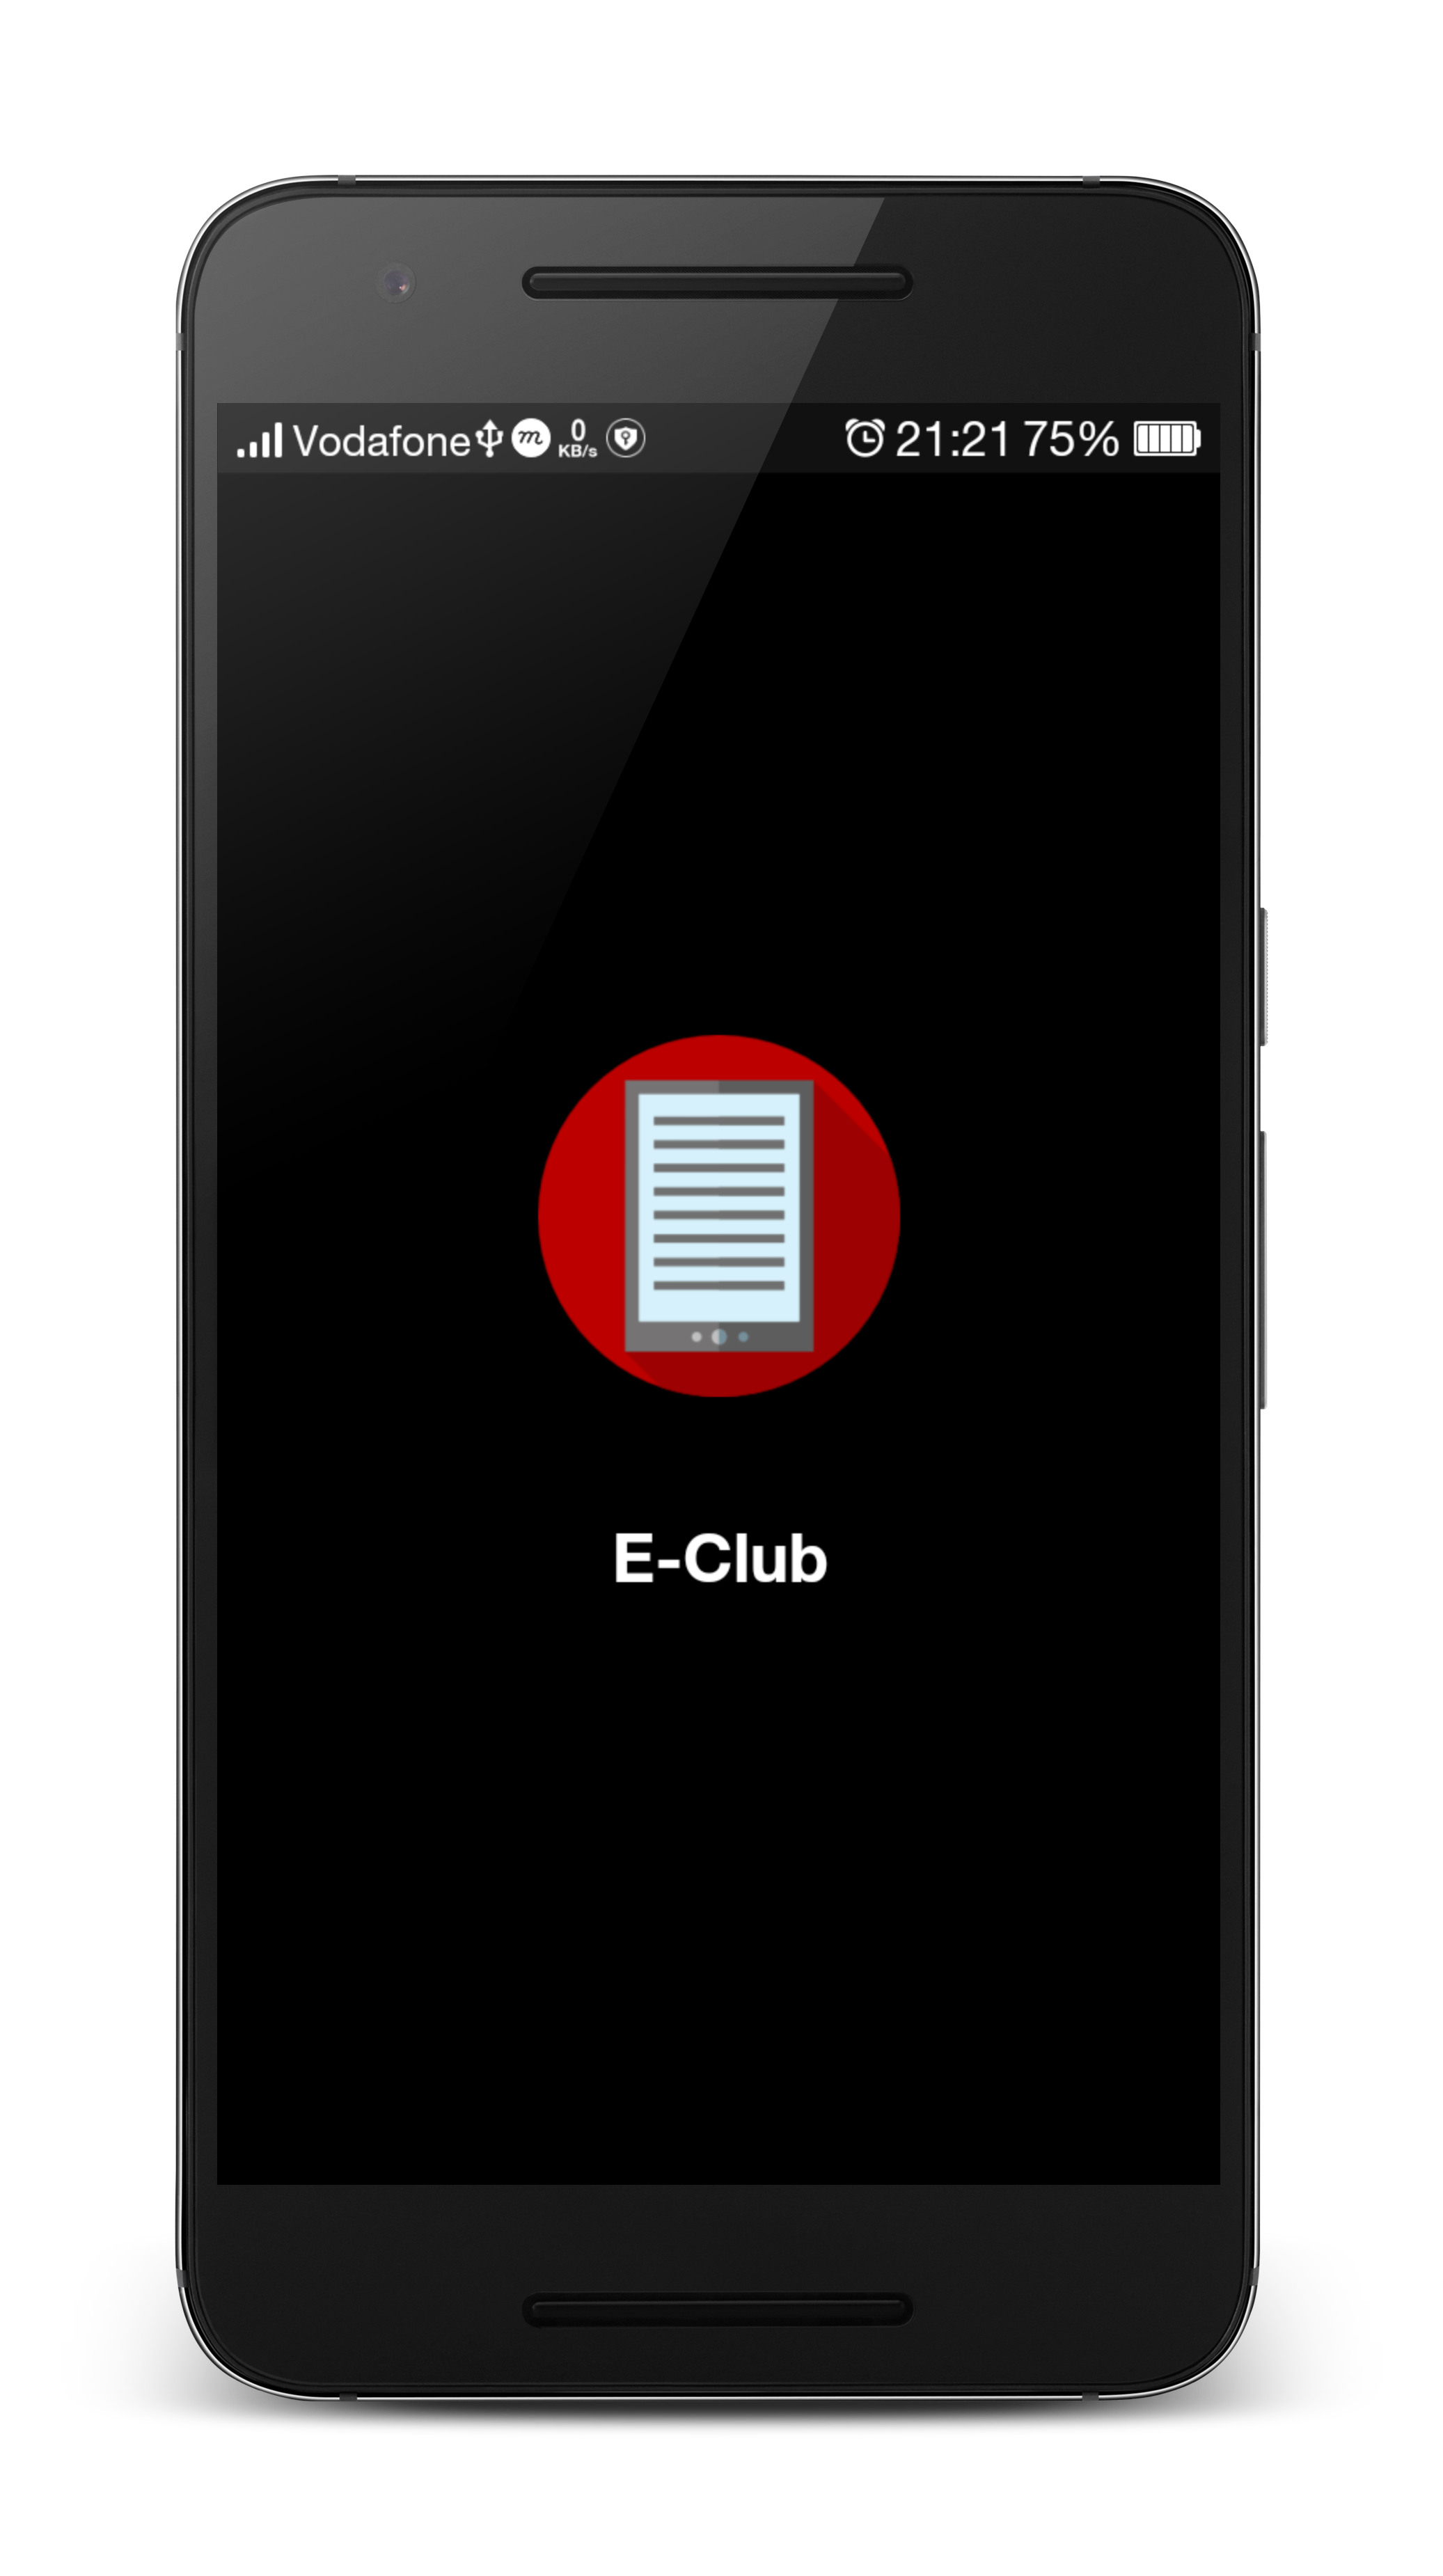
\includegraphics[scale=0.06]{images/d16.png}
\caption{Splash Screen}
\end{figure}

\newpage

%\begin{figure}[ht]
%\centering
%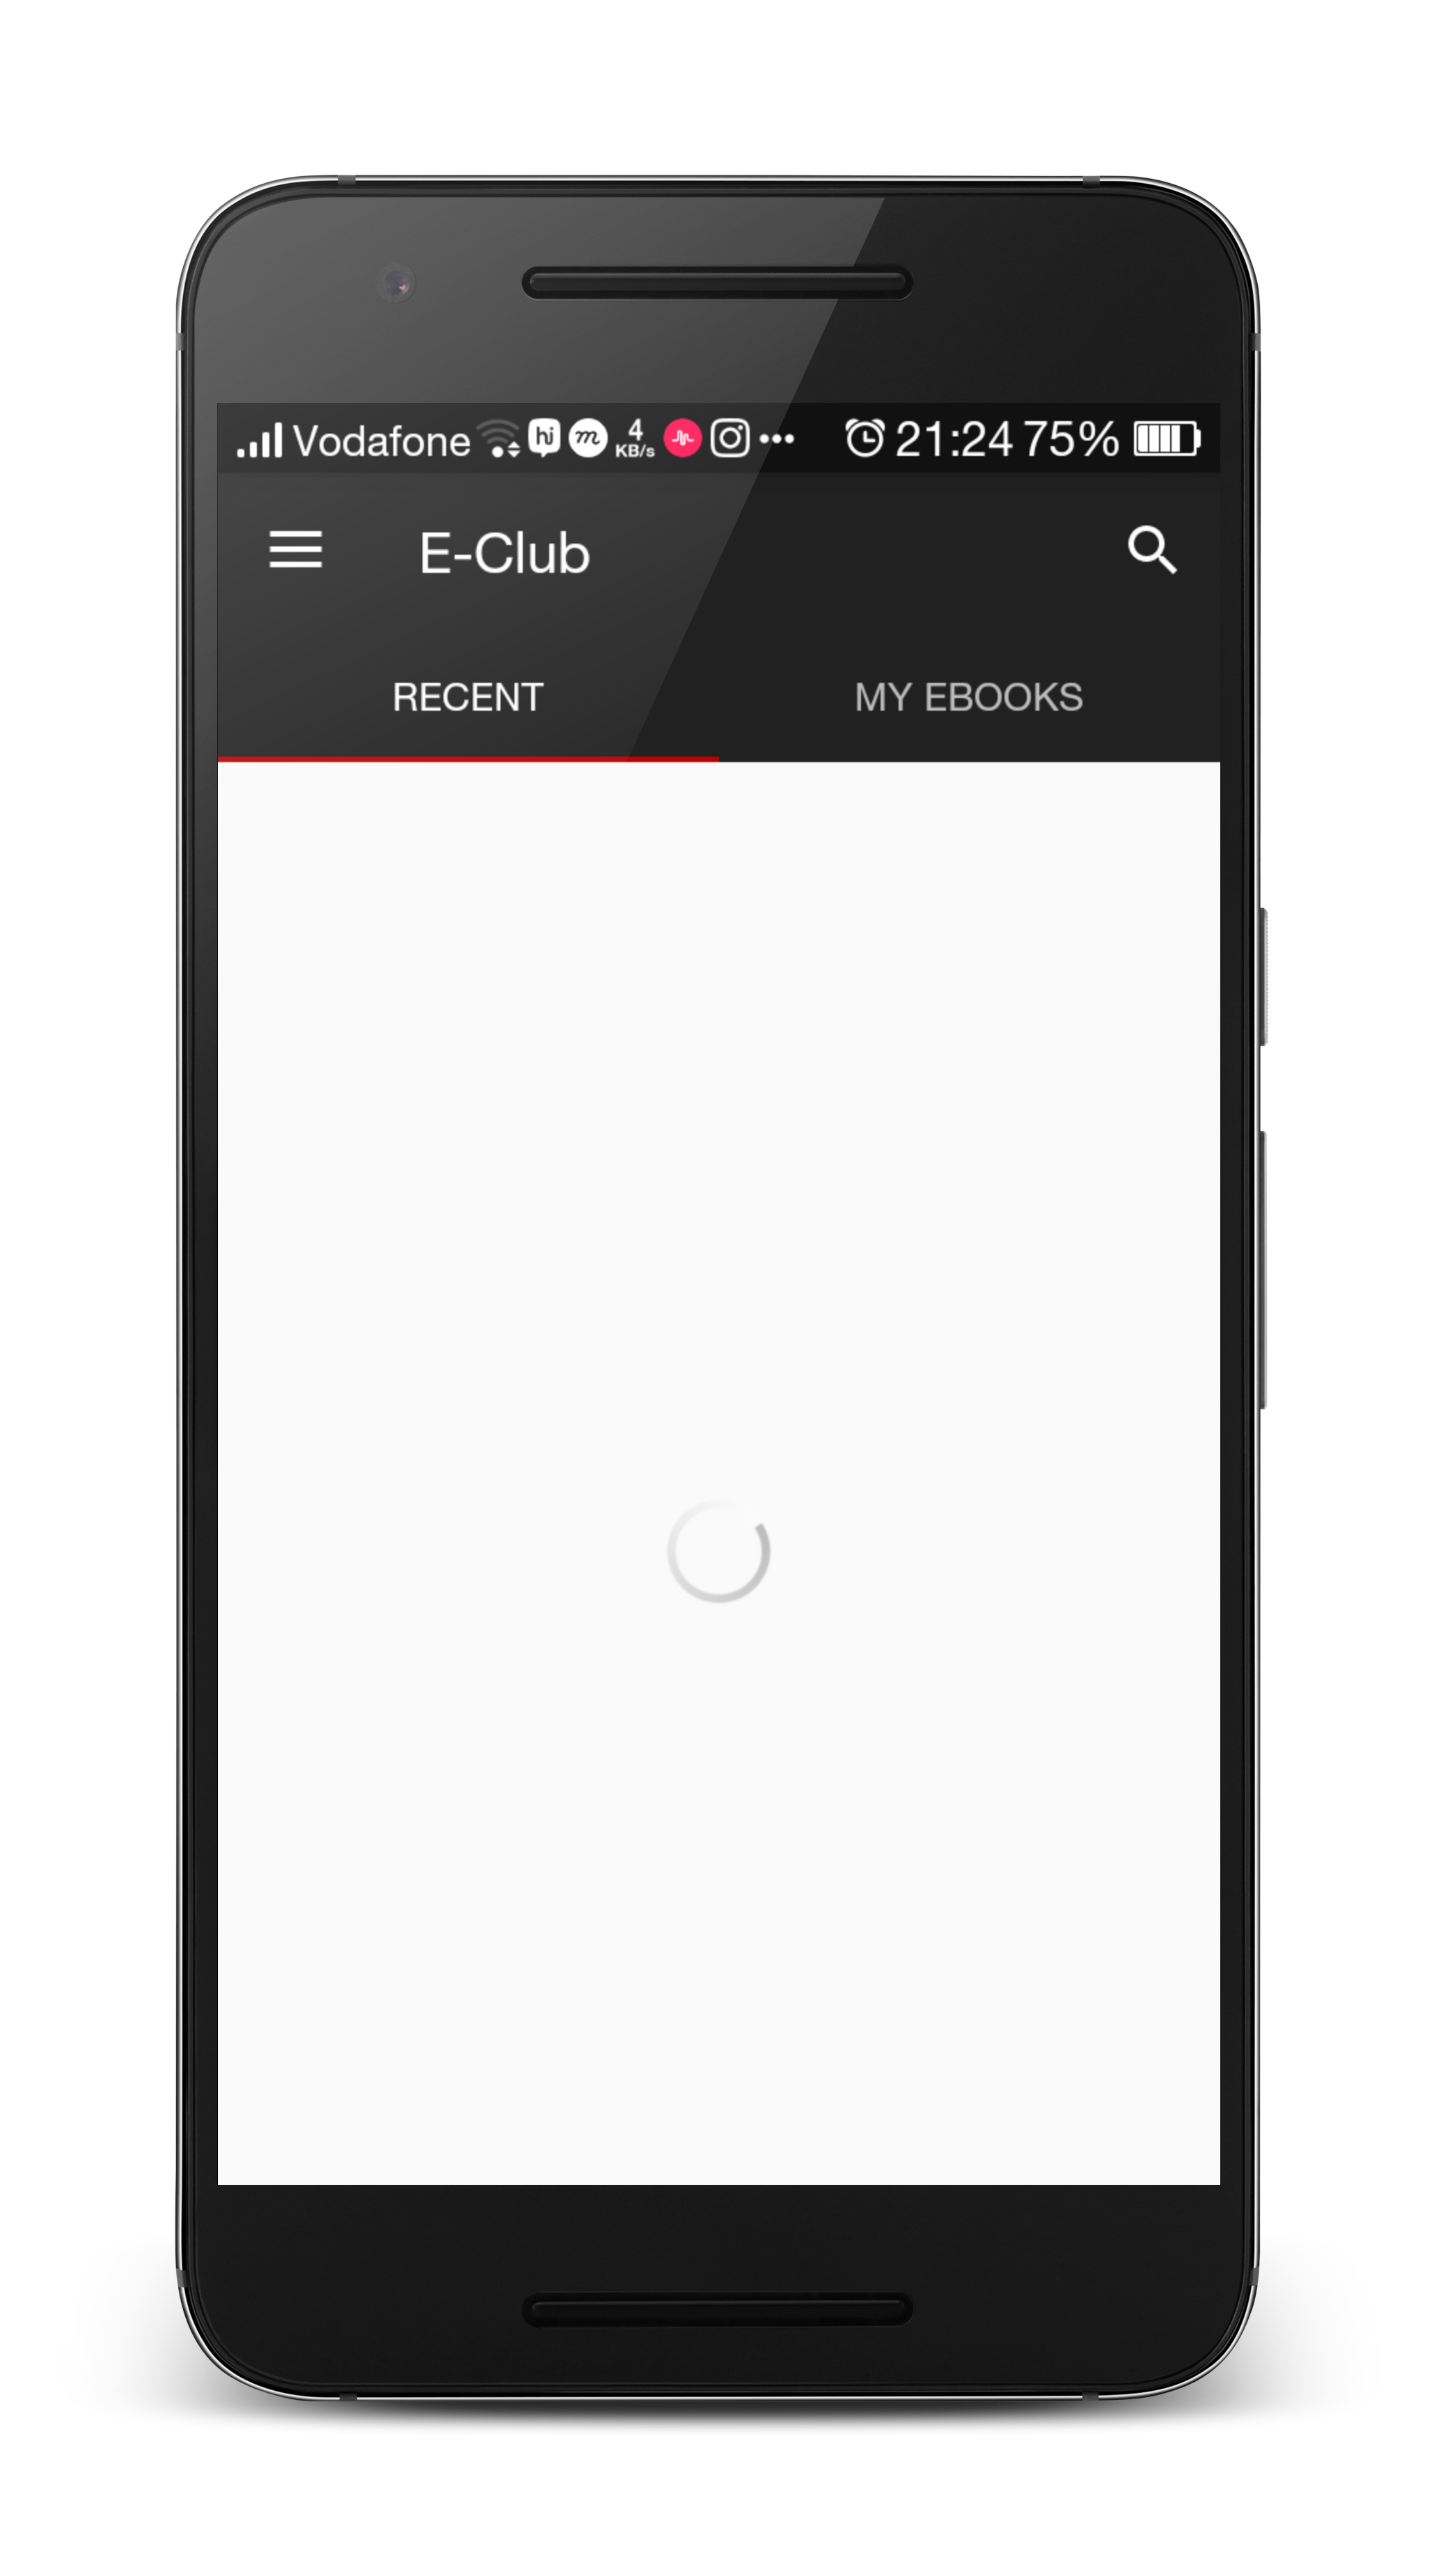
\includegraphics[scale=0.13]{images/d15.png}
%\caption{Screen 2}
%\end{figure}

%\newpage

\begin{figure}[ht]
\centering
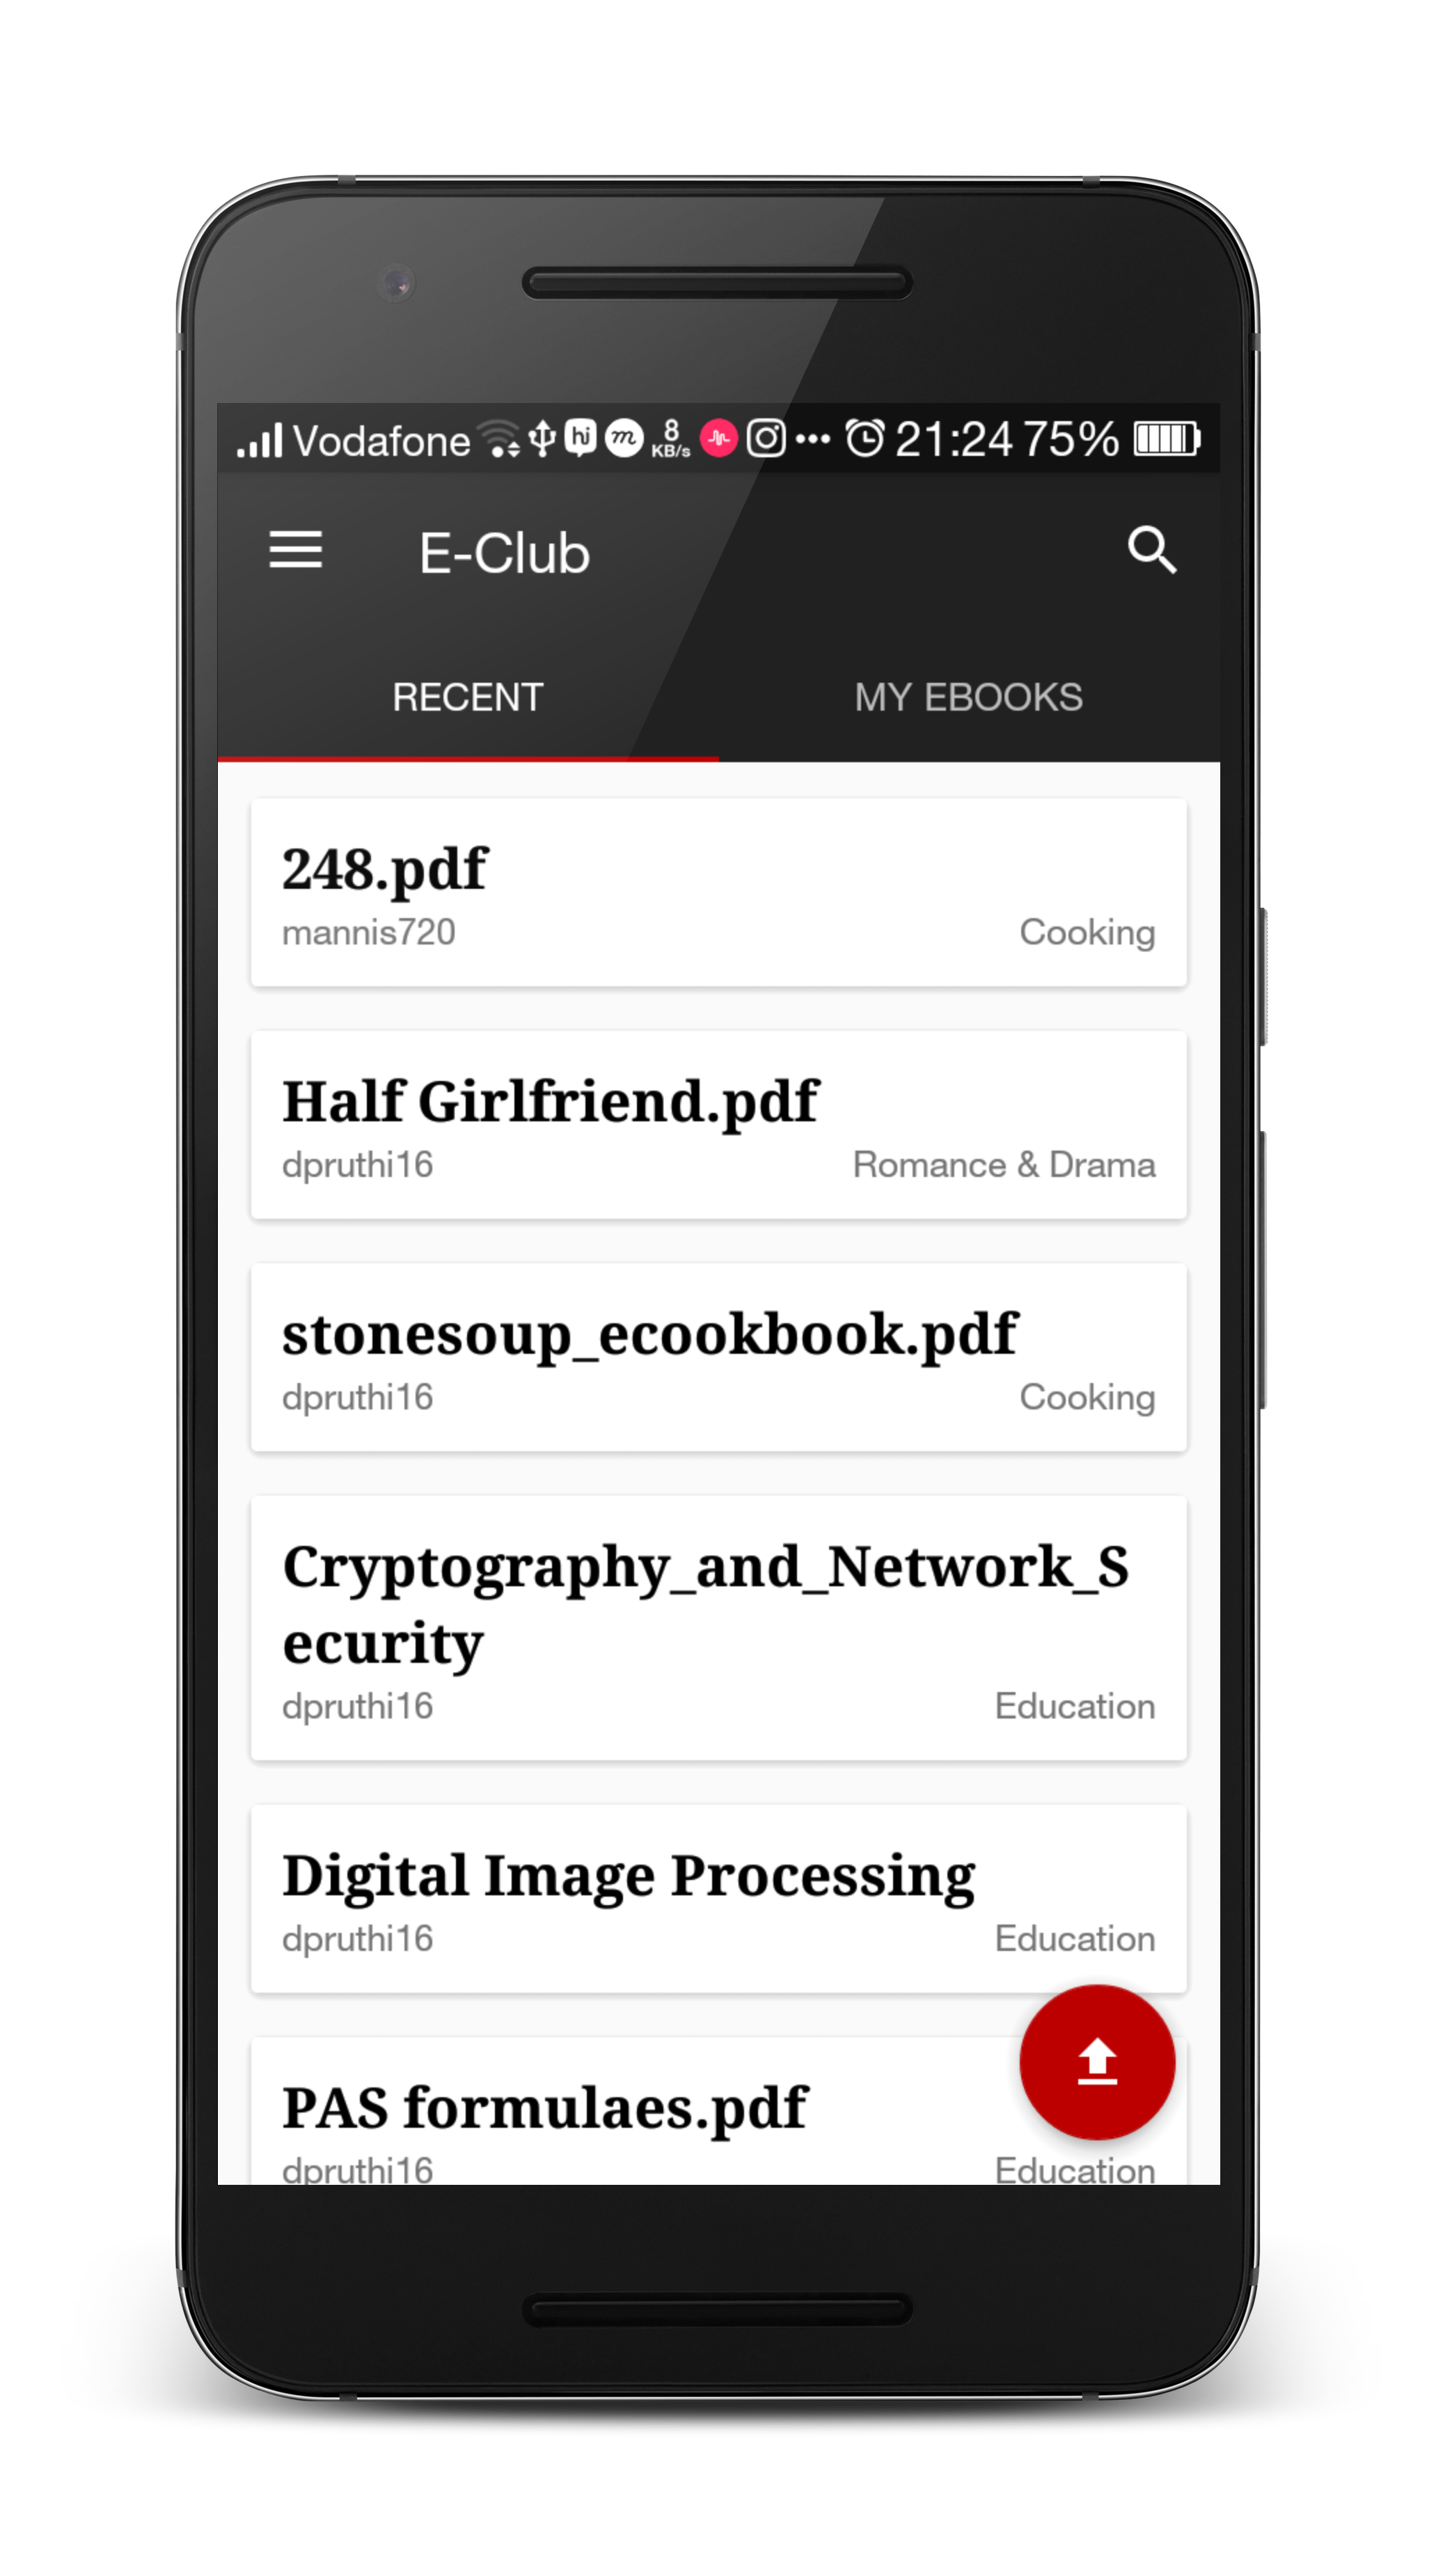
\includegraphics[scale=0.13]{images/d14.png}
\caption{Recent Ebooks Uploaded}
\end{figure}

\newpage

\begin{figure}[ht]
\centering
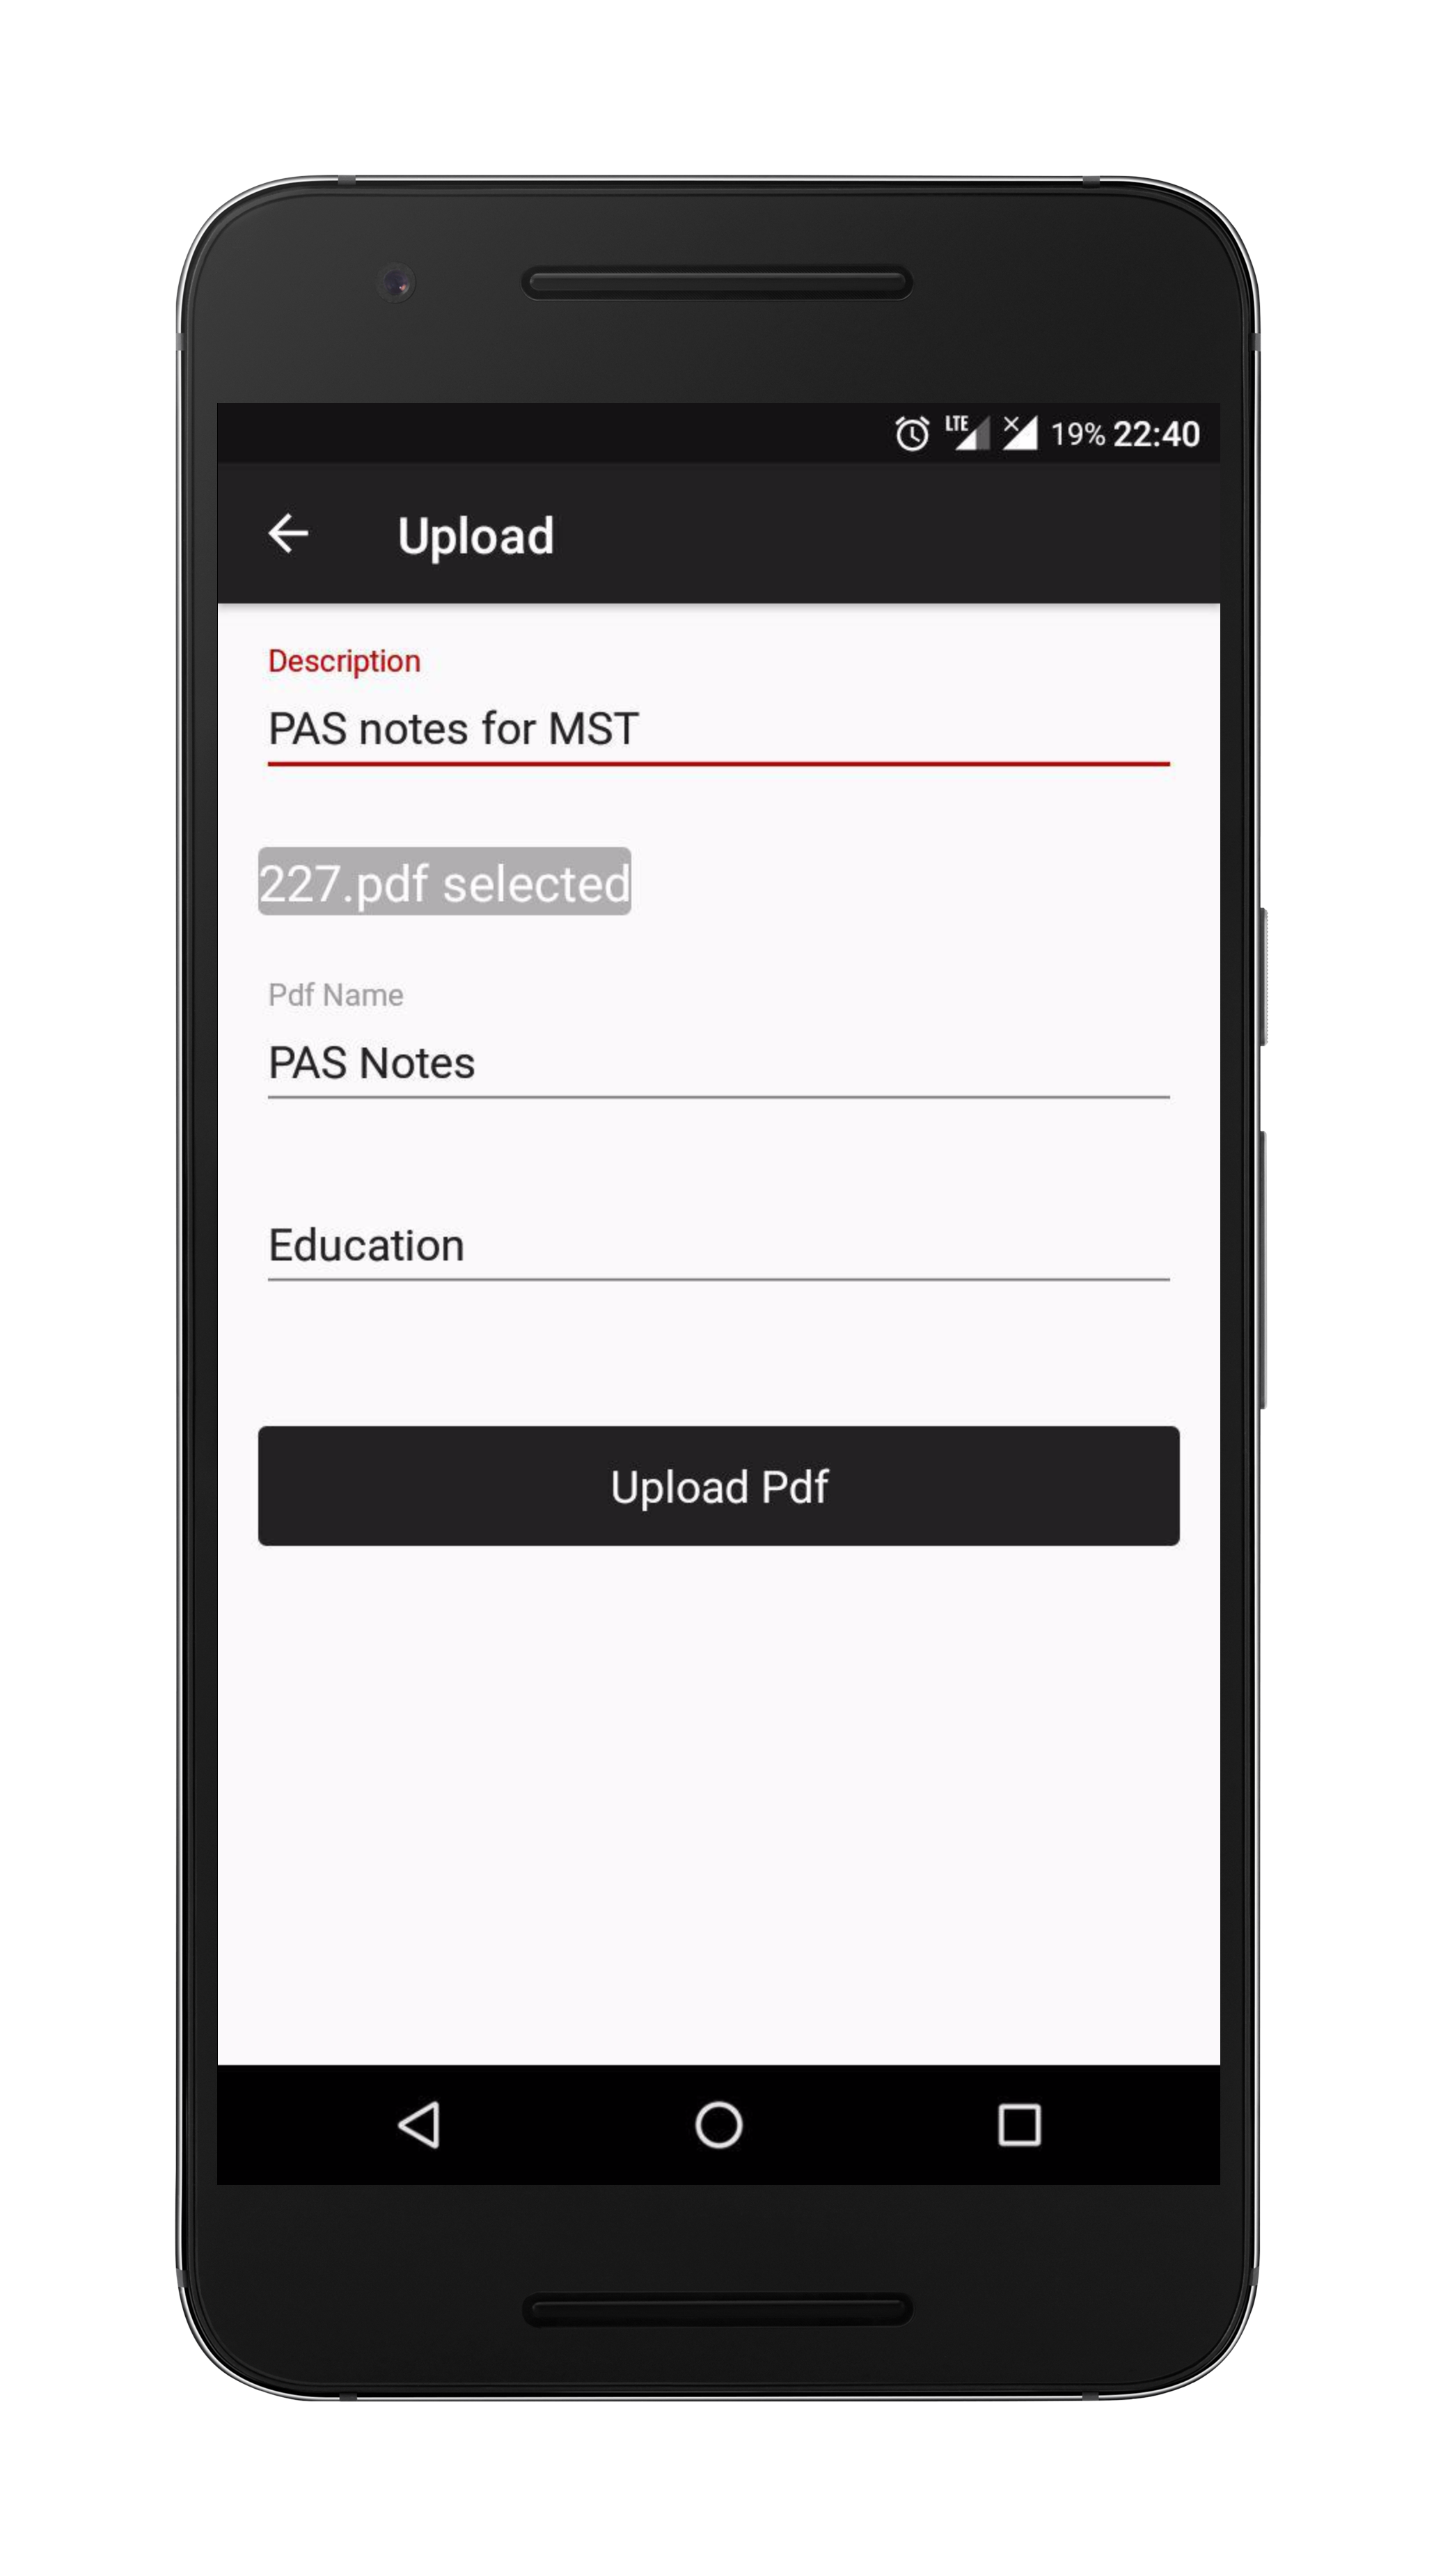
\includegraphics[scale=0.13]{images/up.png}
\caption{Uploading Ebook}
\end{figure}

\newpage

\begin{figure}[ht]
\centering
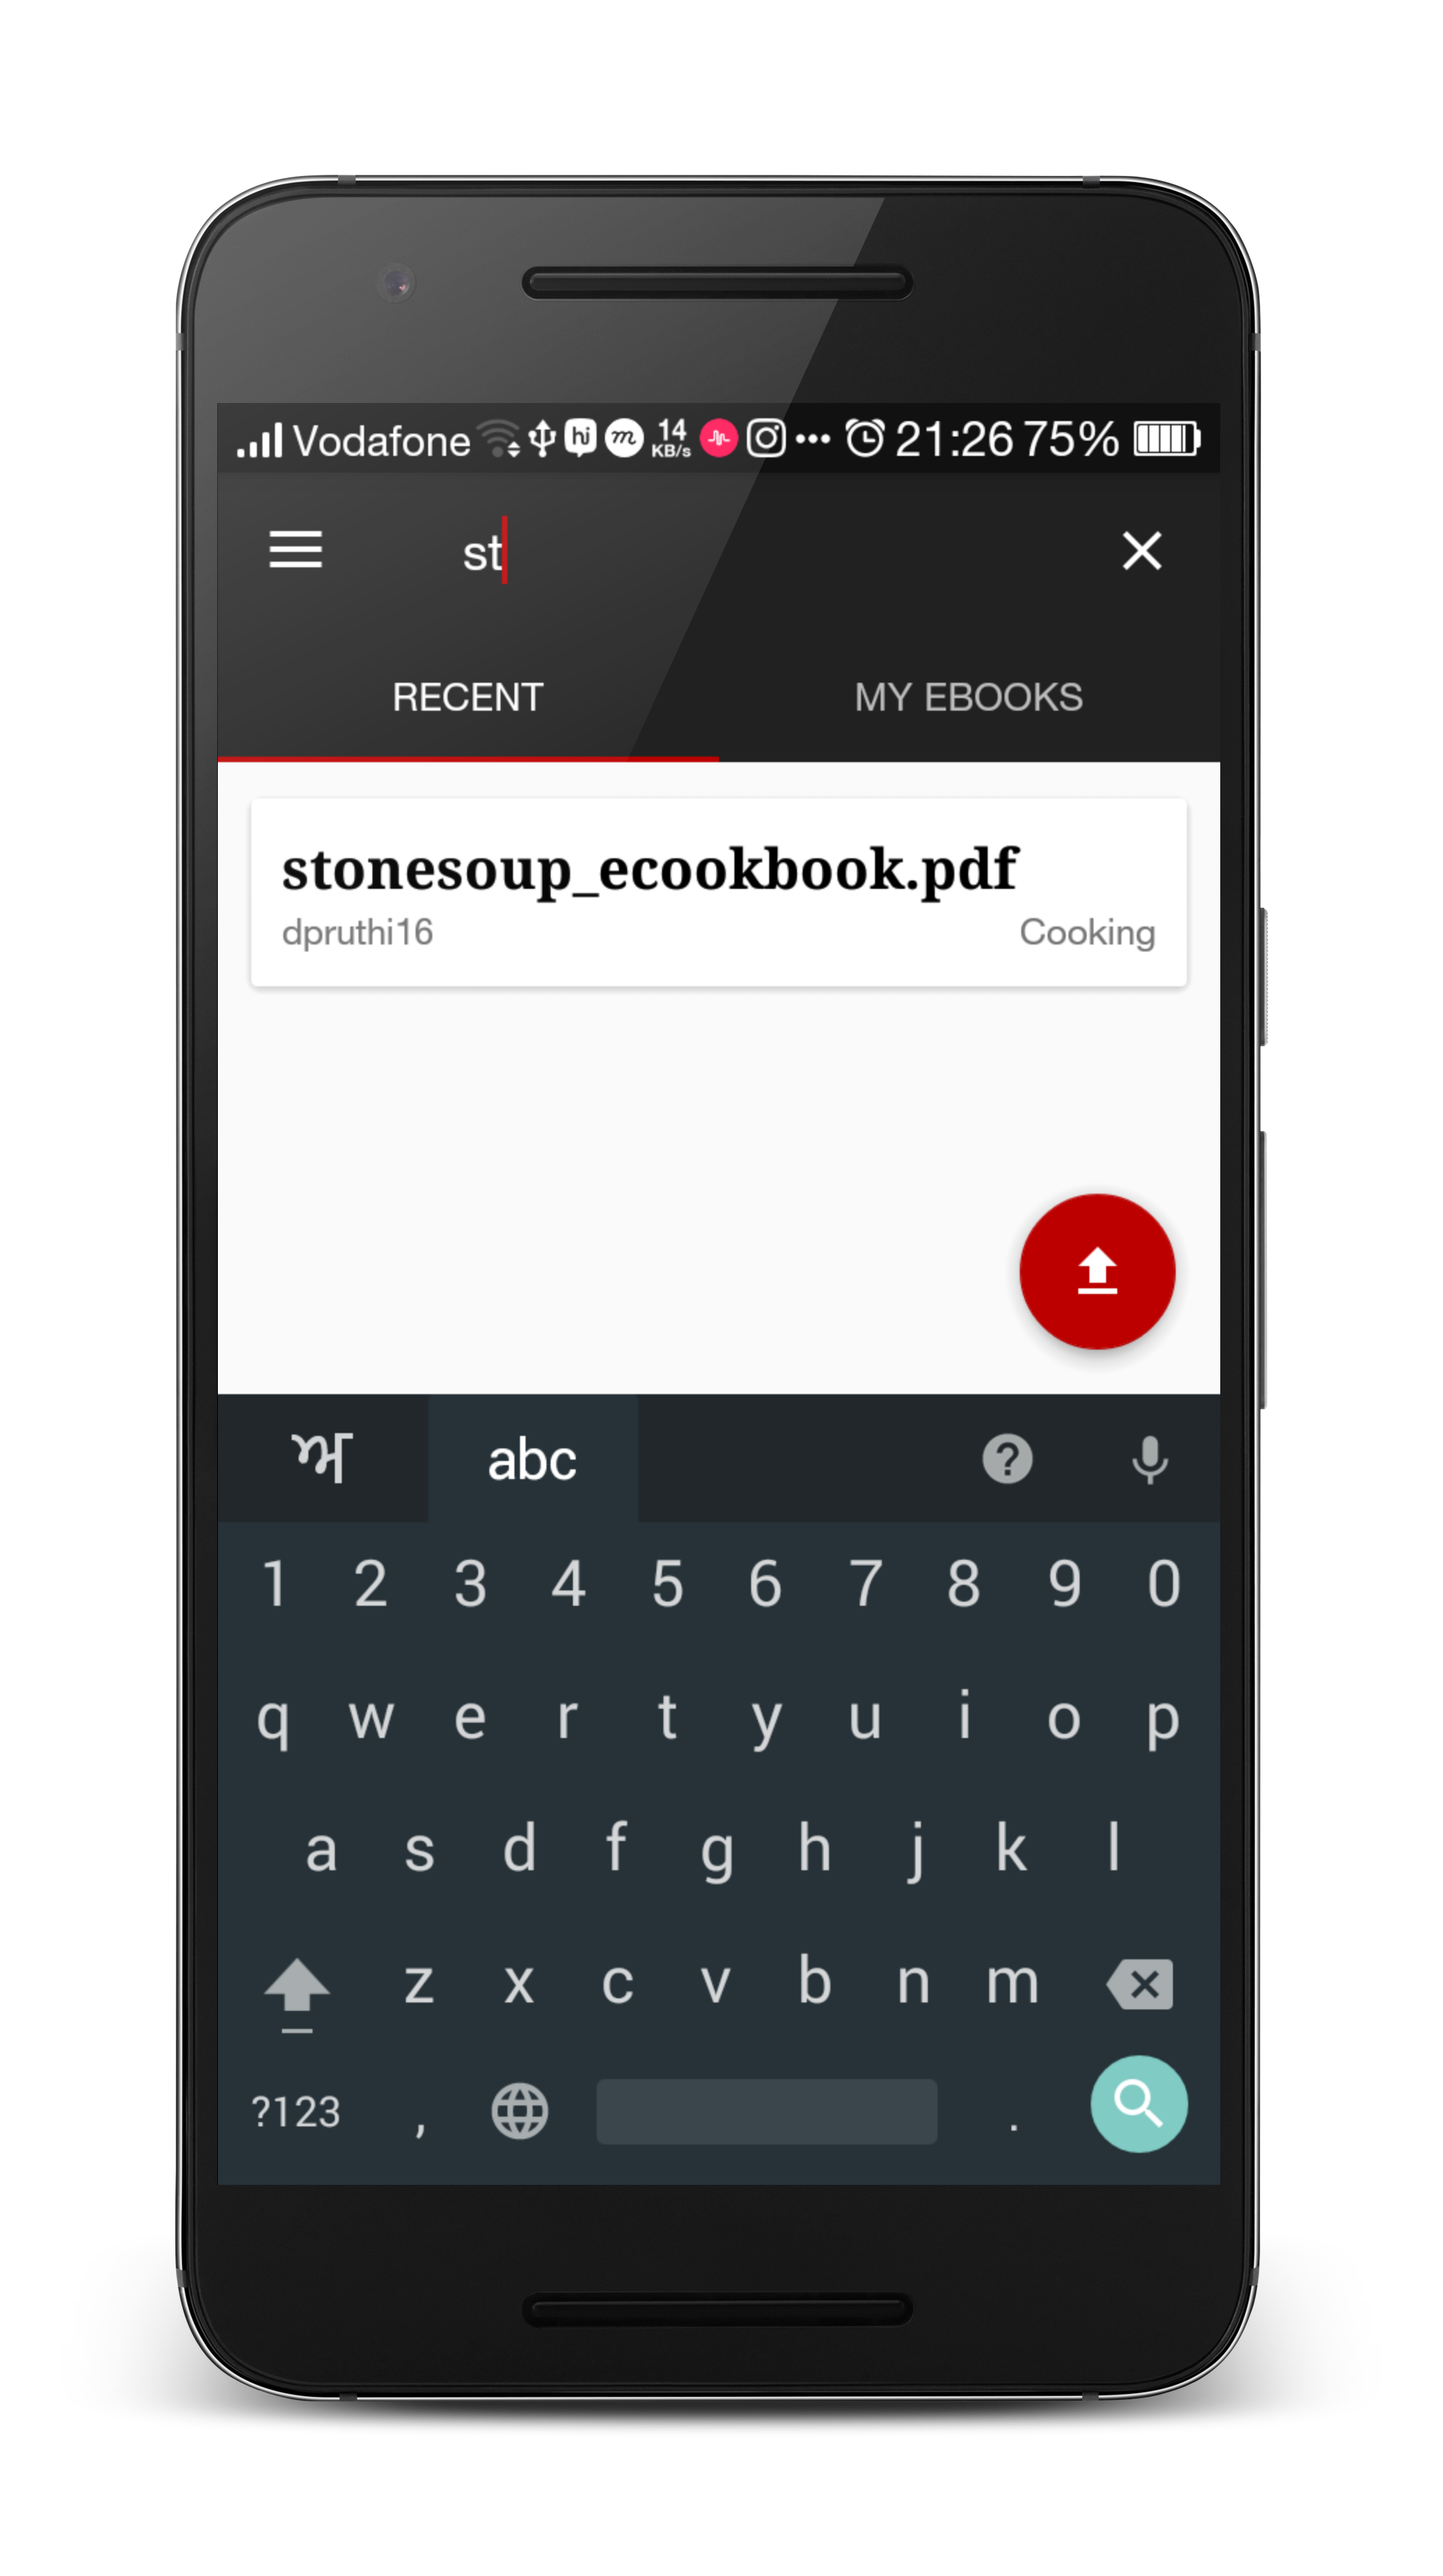
\includegraphics[scale=0.13]{images/d10.png}
\caption{Searching Ebook}
\end{figure}

\newpage

\begin{figure}[ht]
\centering
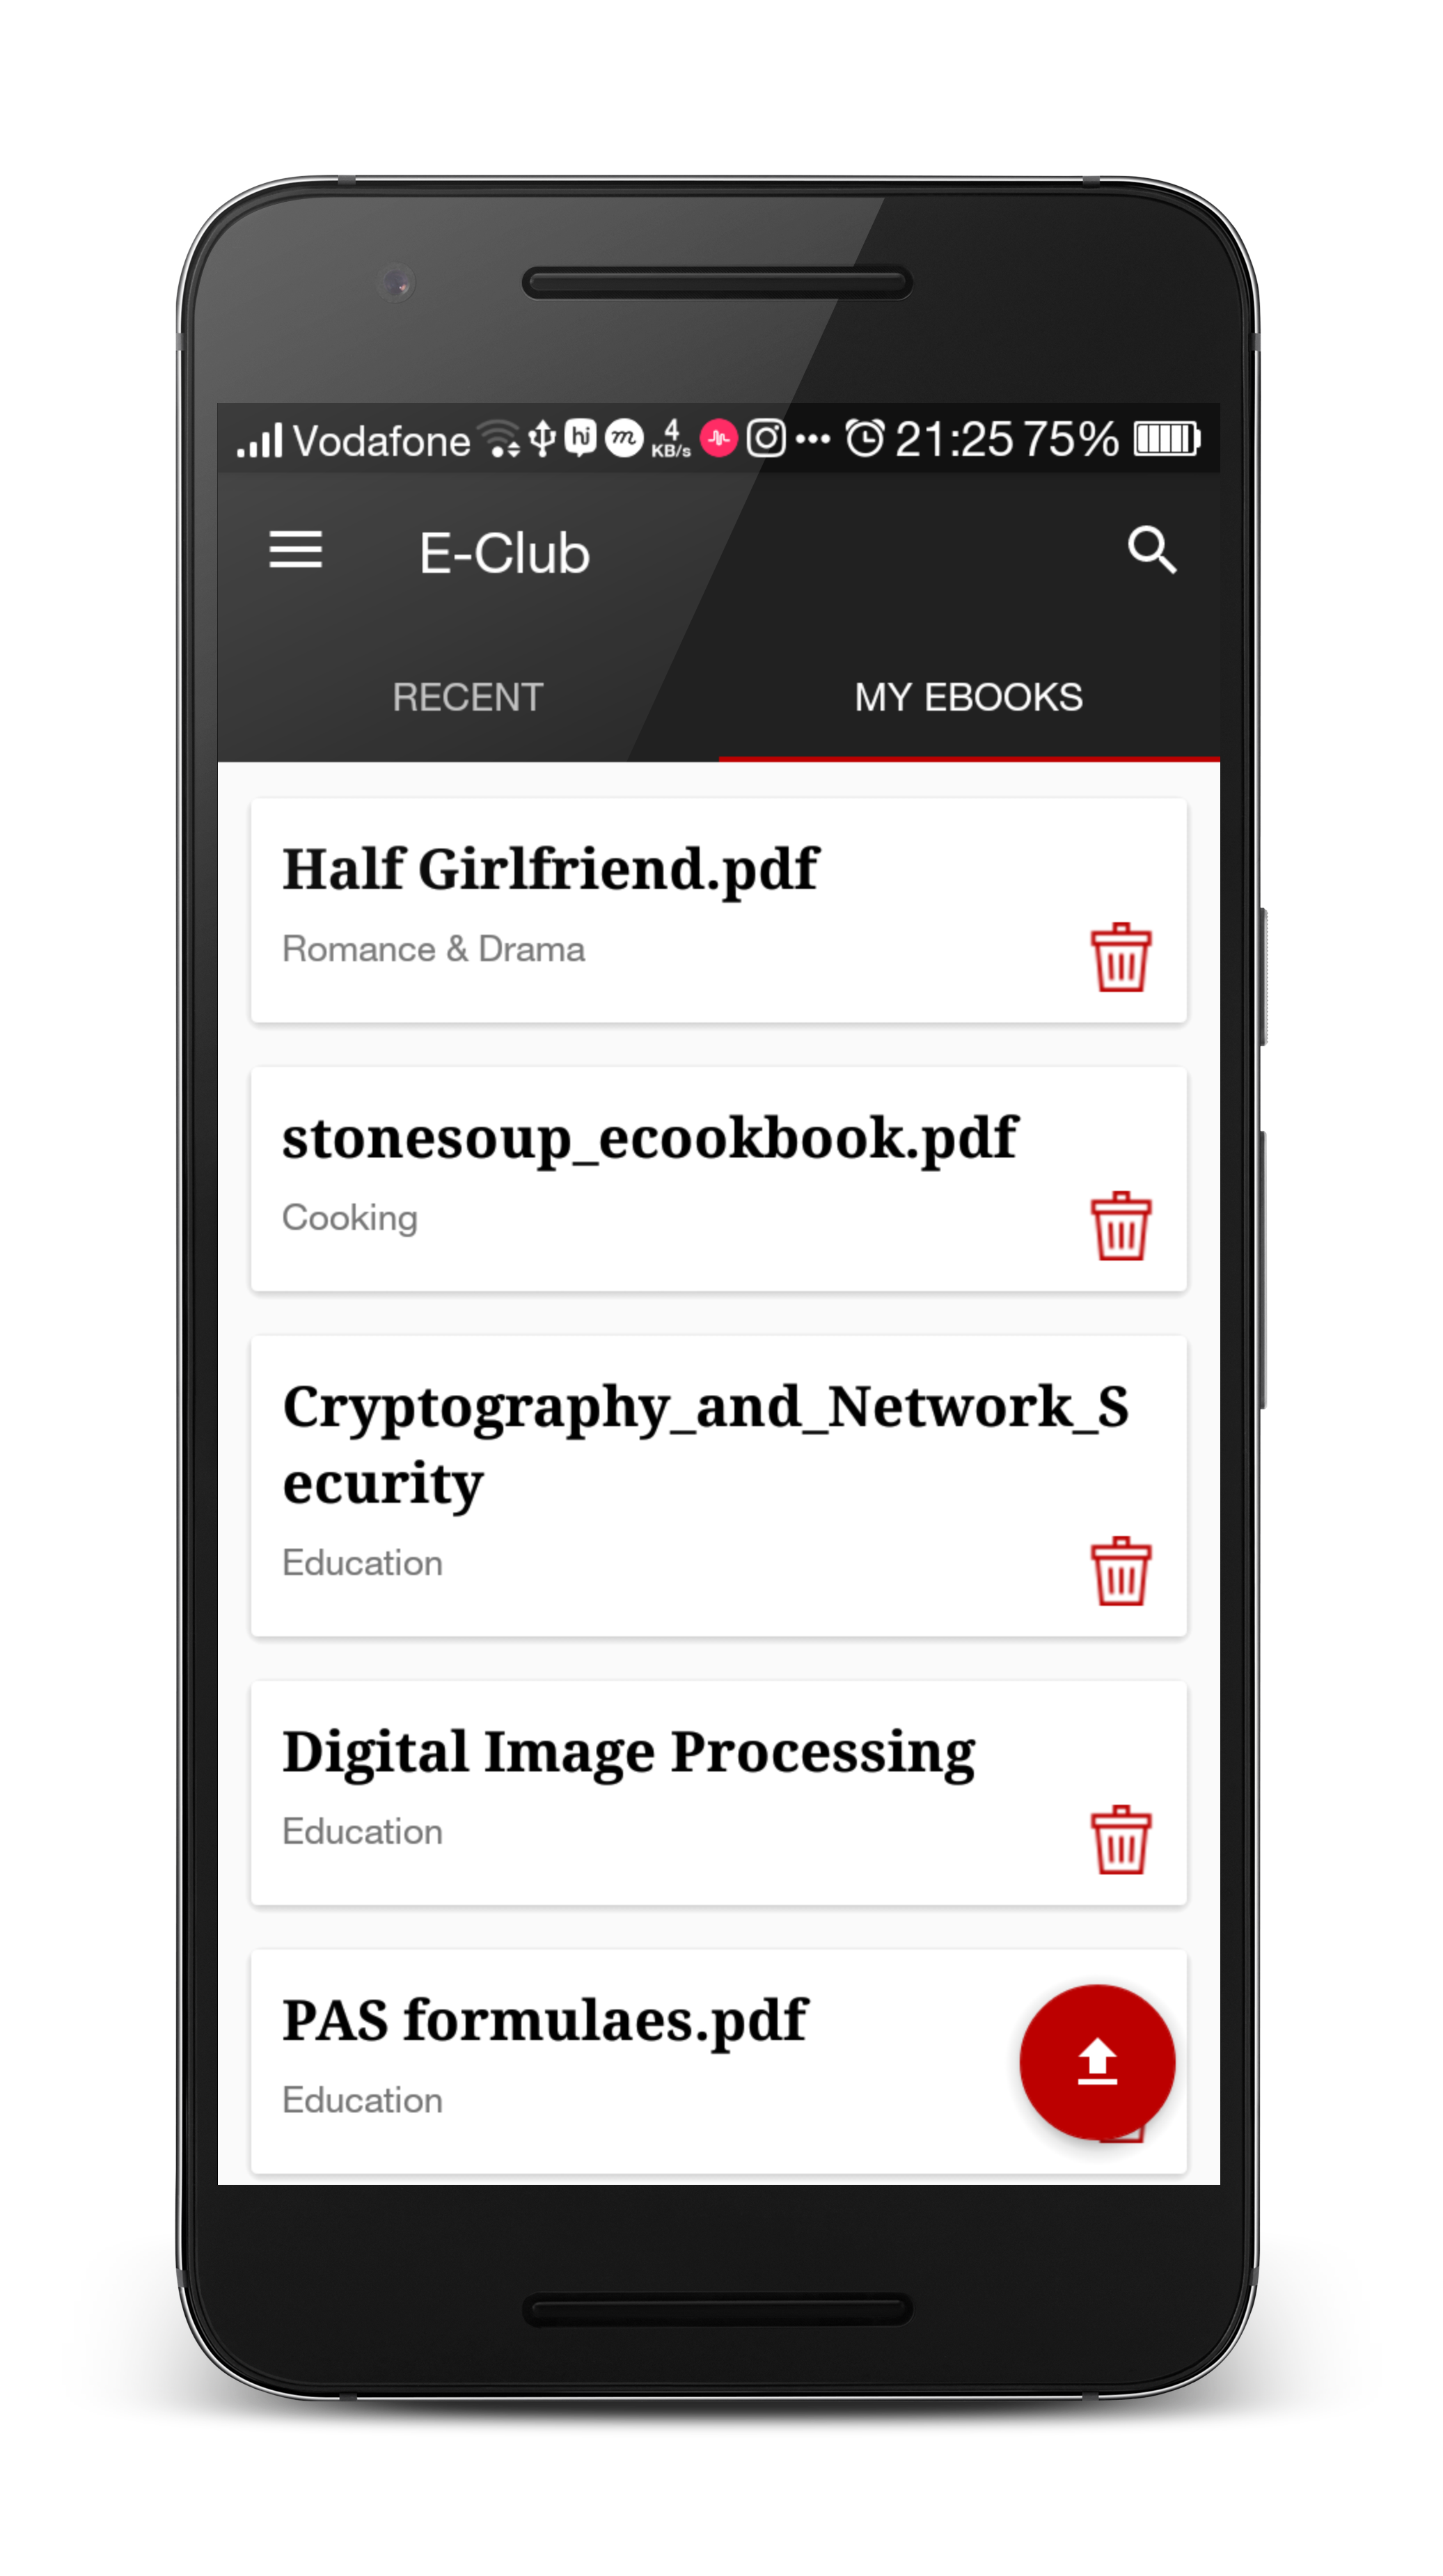
\includegraphics[scale=0.13]{images/d12.png}
\caption{My Ebooks}
\end{figure}

\newpage

%\begin{figure}[ht]
%\centering
%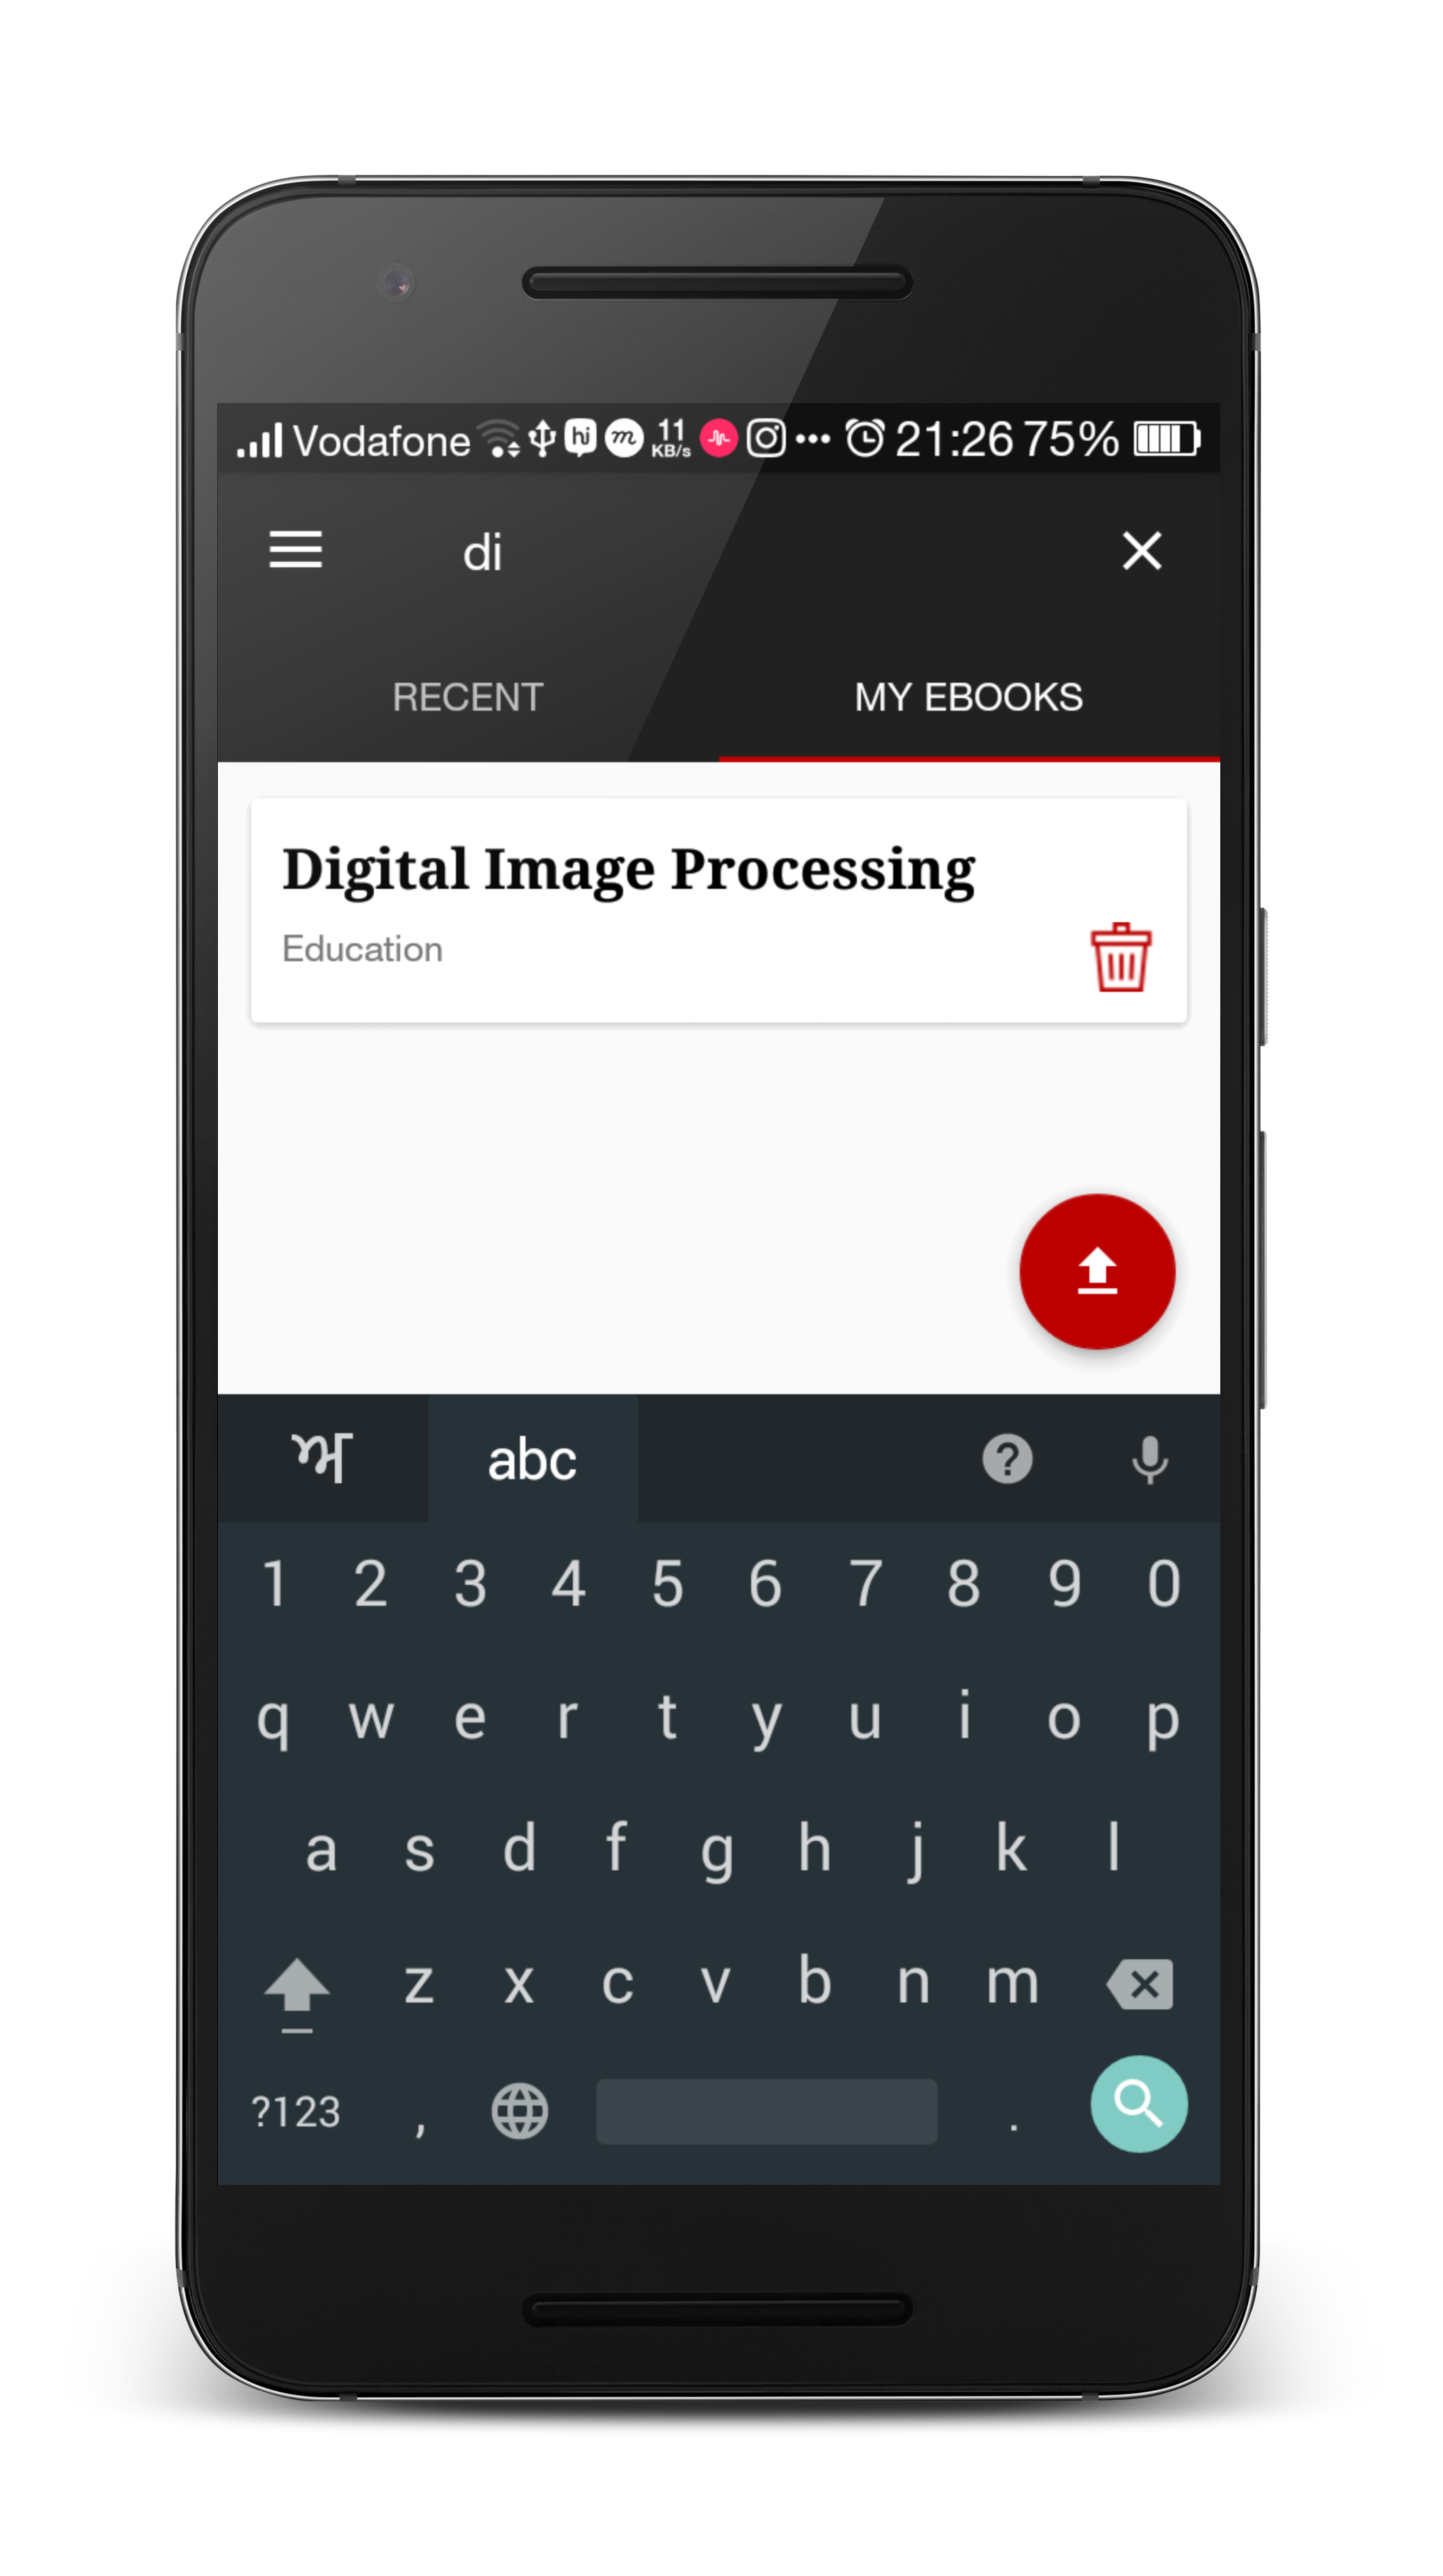
\includegraphics[scale=0.13]{images/d11.png}
%\caption{Screen 7}
%\end{figure}

%\newpage

\begin{figure}[ht]
\centering
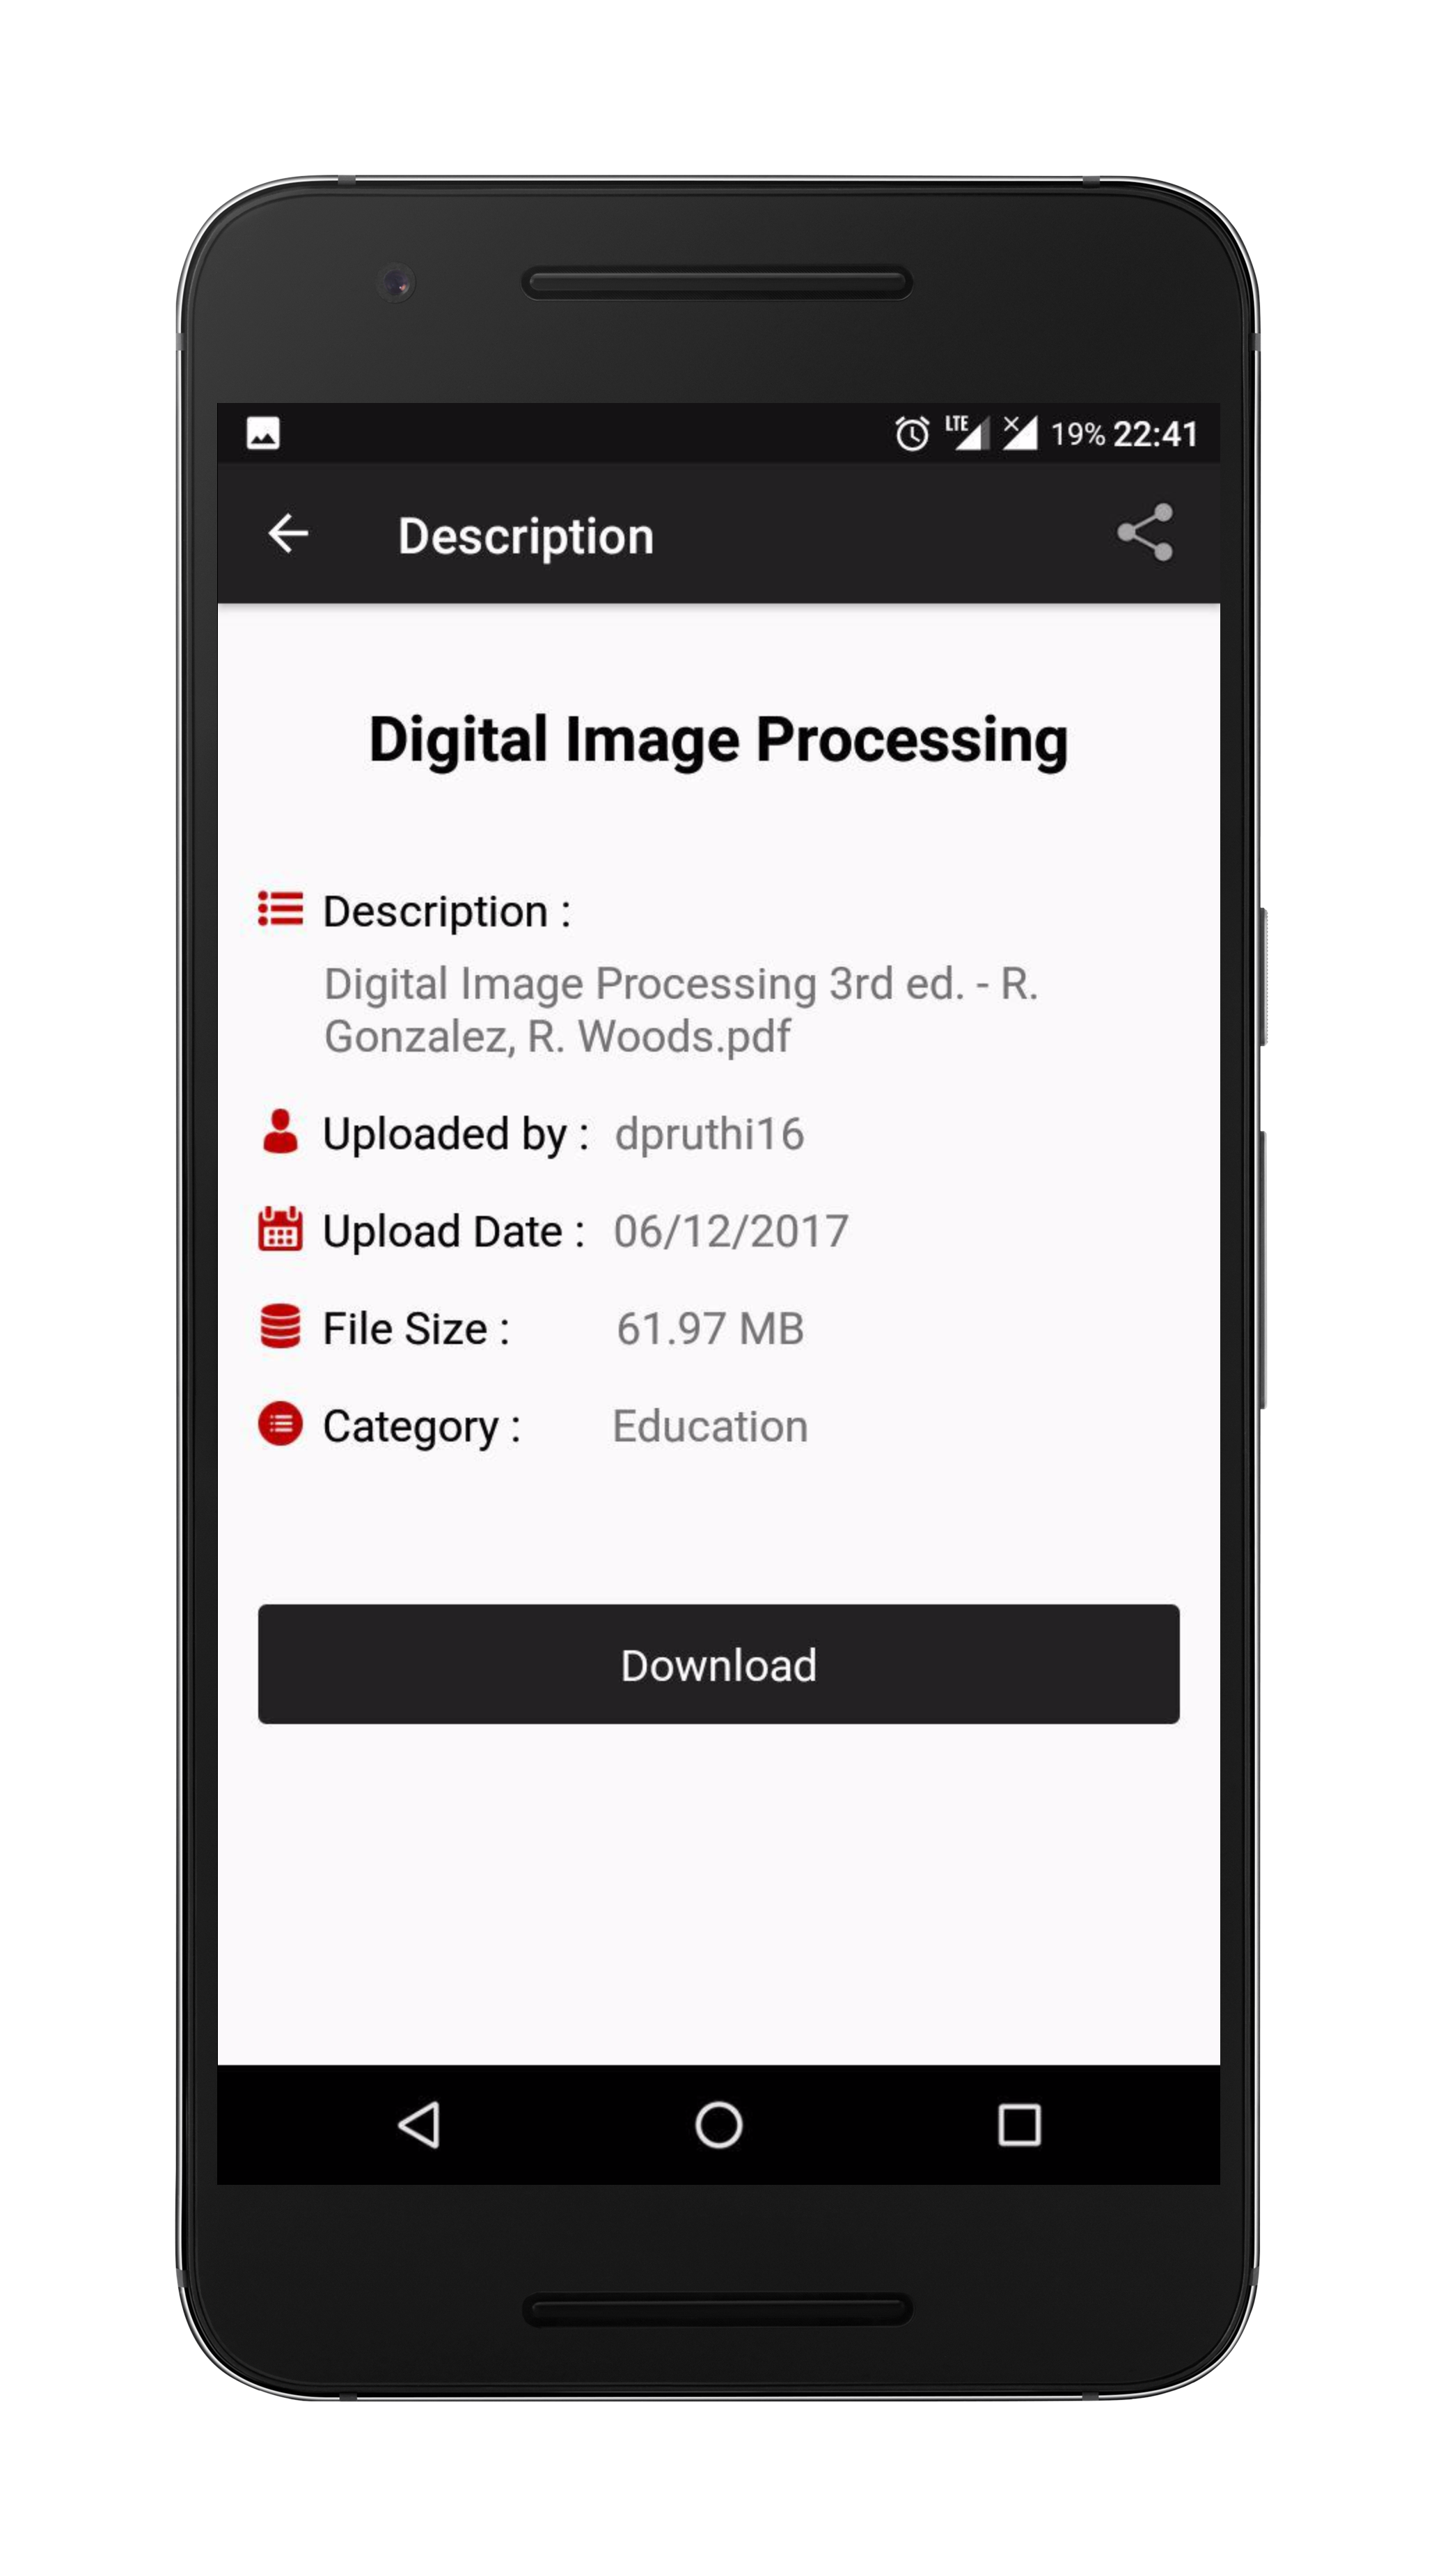
\includegraphics[scale=0.13]{images/de.png}
\caption{Ebook Description}
\end{figure}

\newpage

\begin{figure}[ht]
\centering
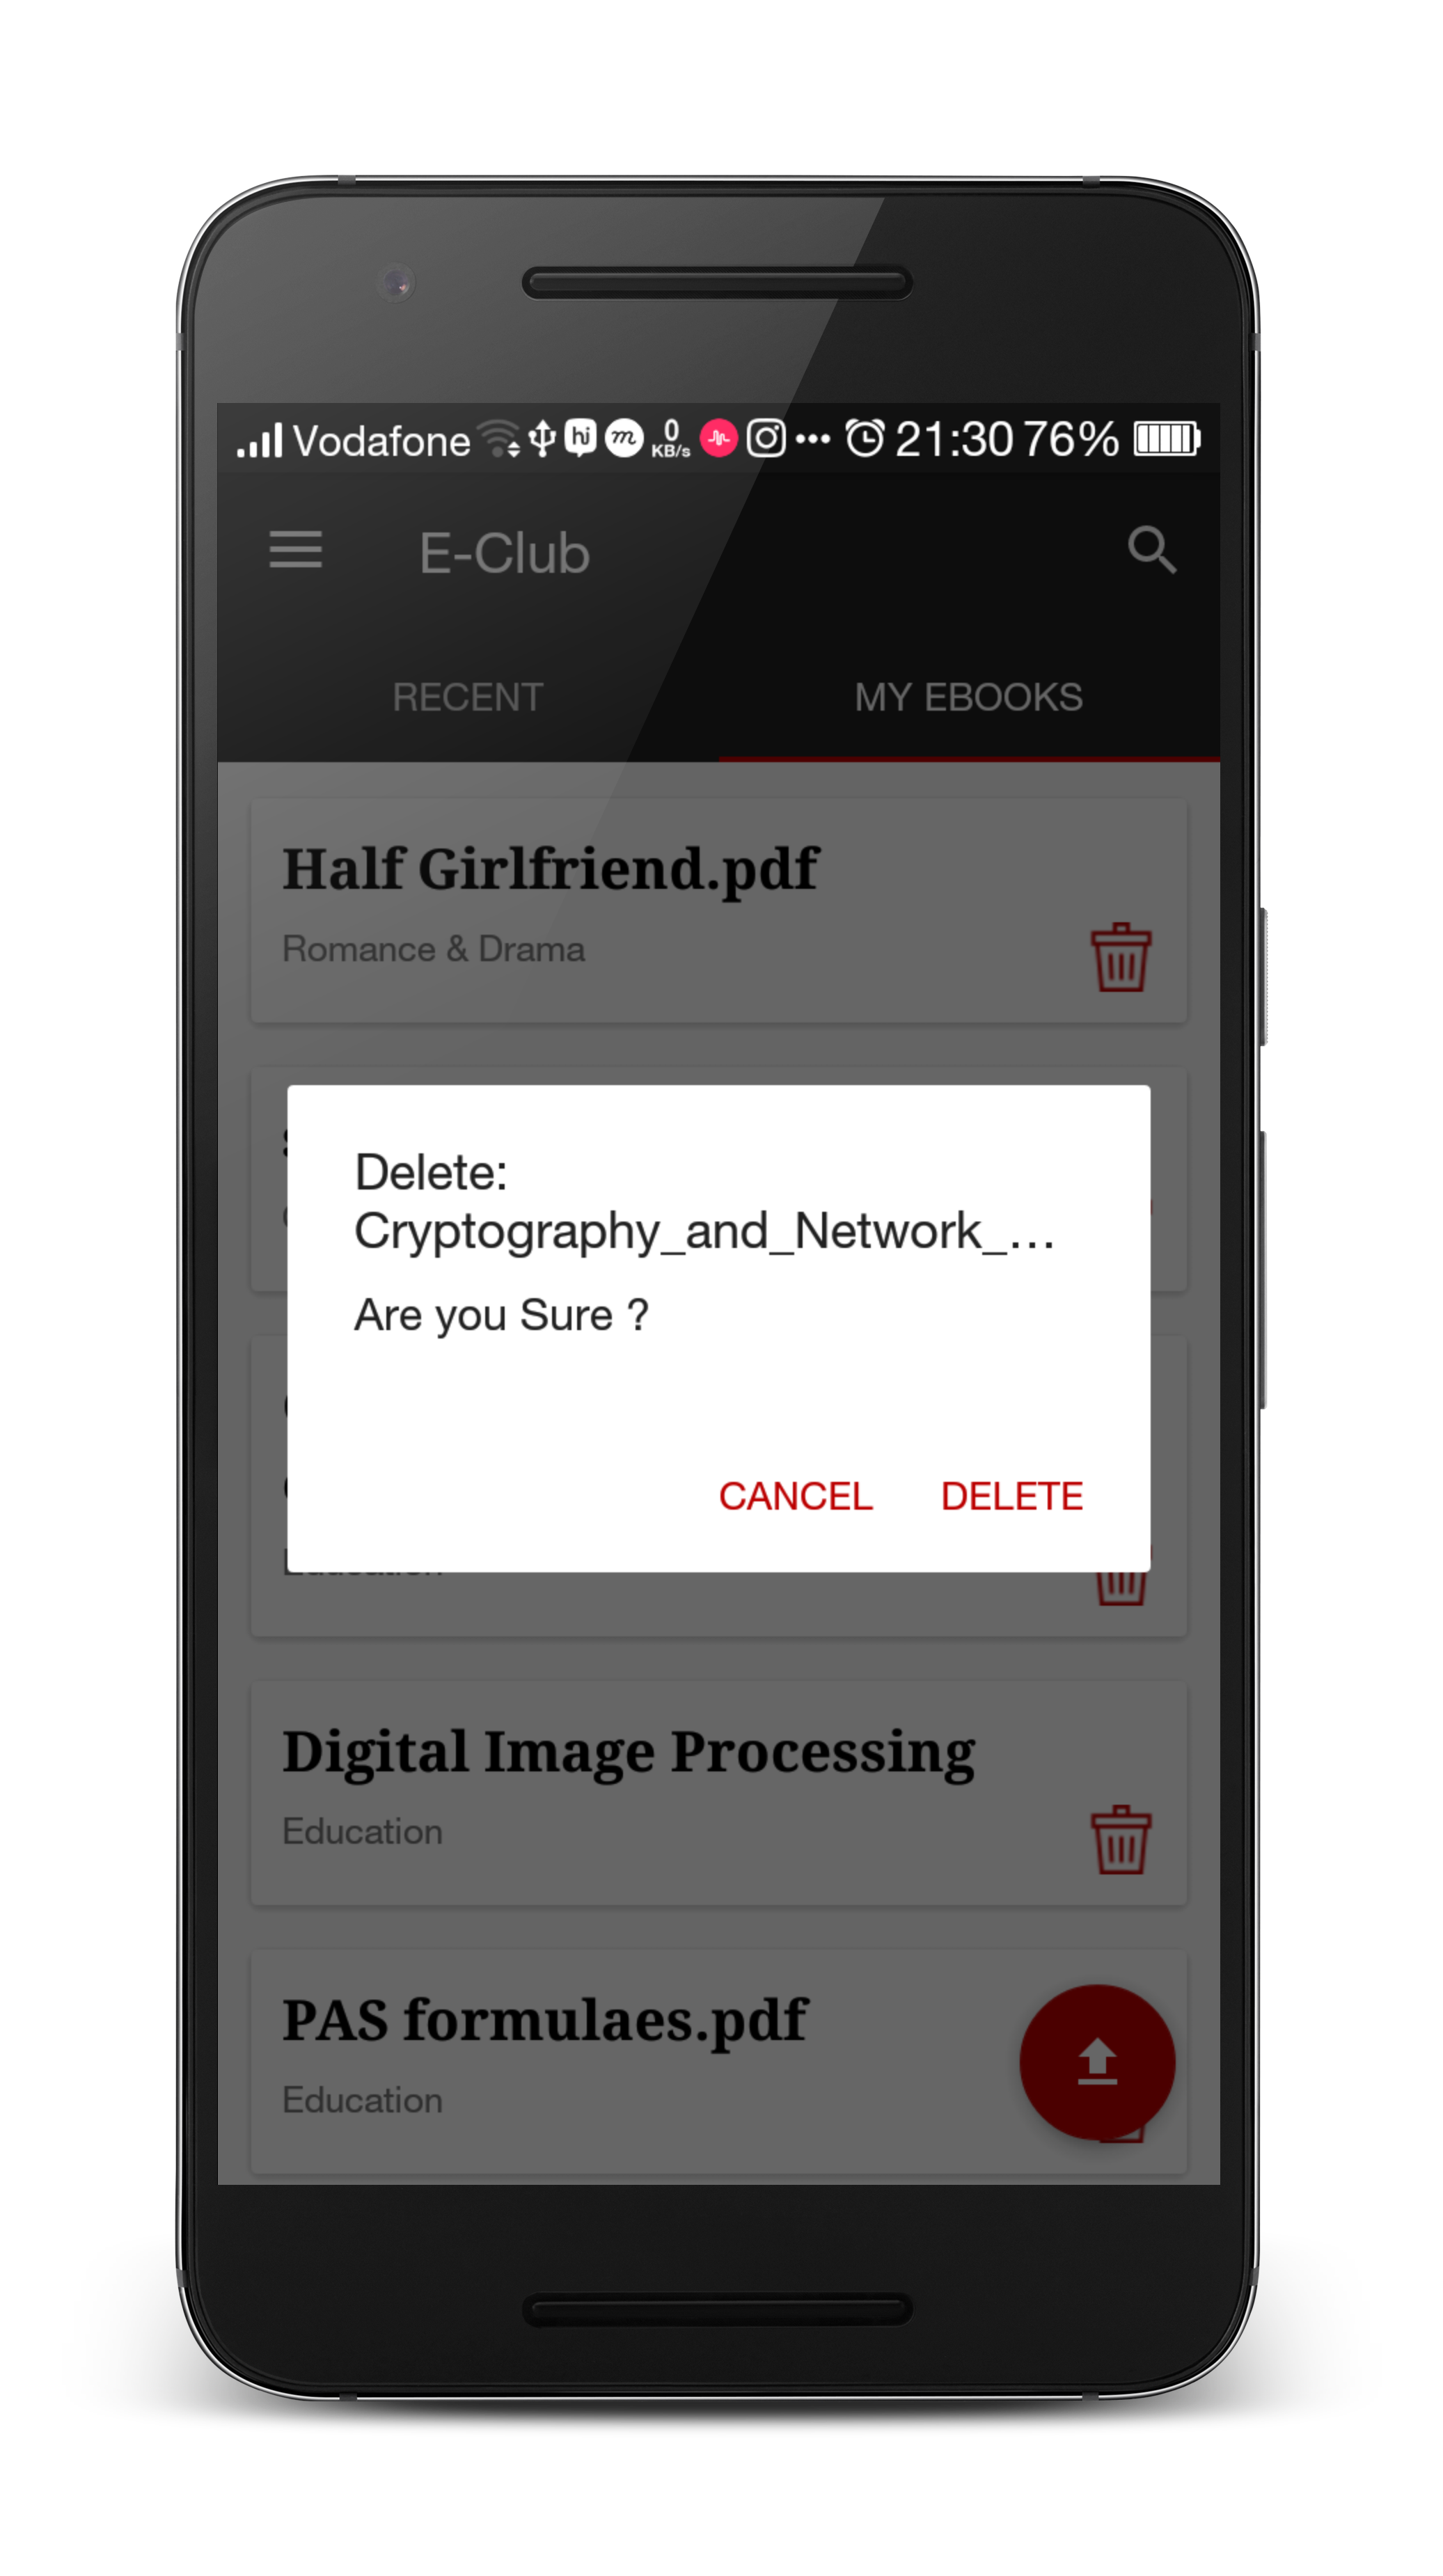
\includegraphics[scale=0.13]{images/d1.png}
\caption{Deleting Ebook}
\end{figure}

\newpage

\begin{figure}[ht]
\centering
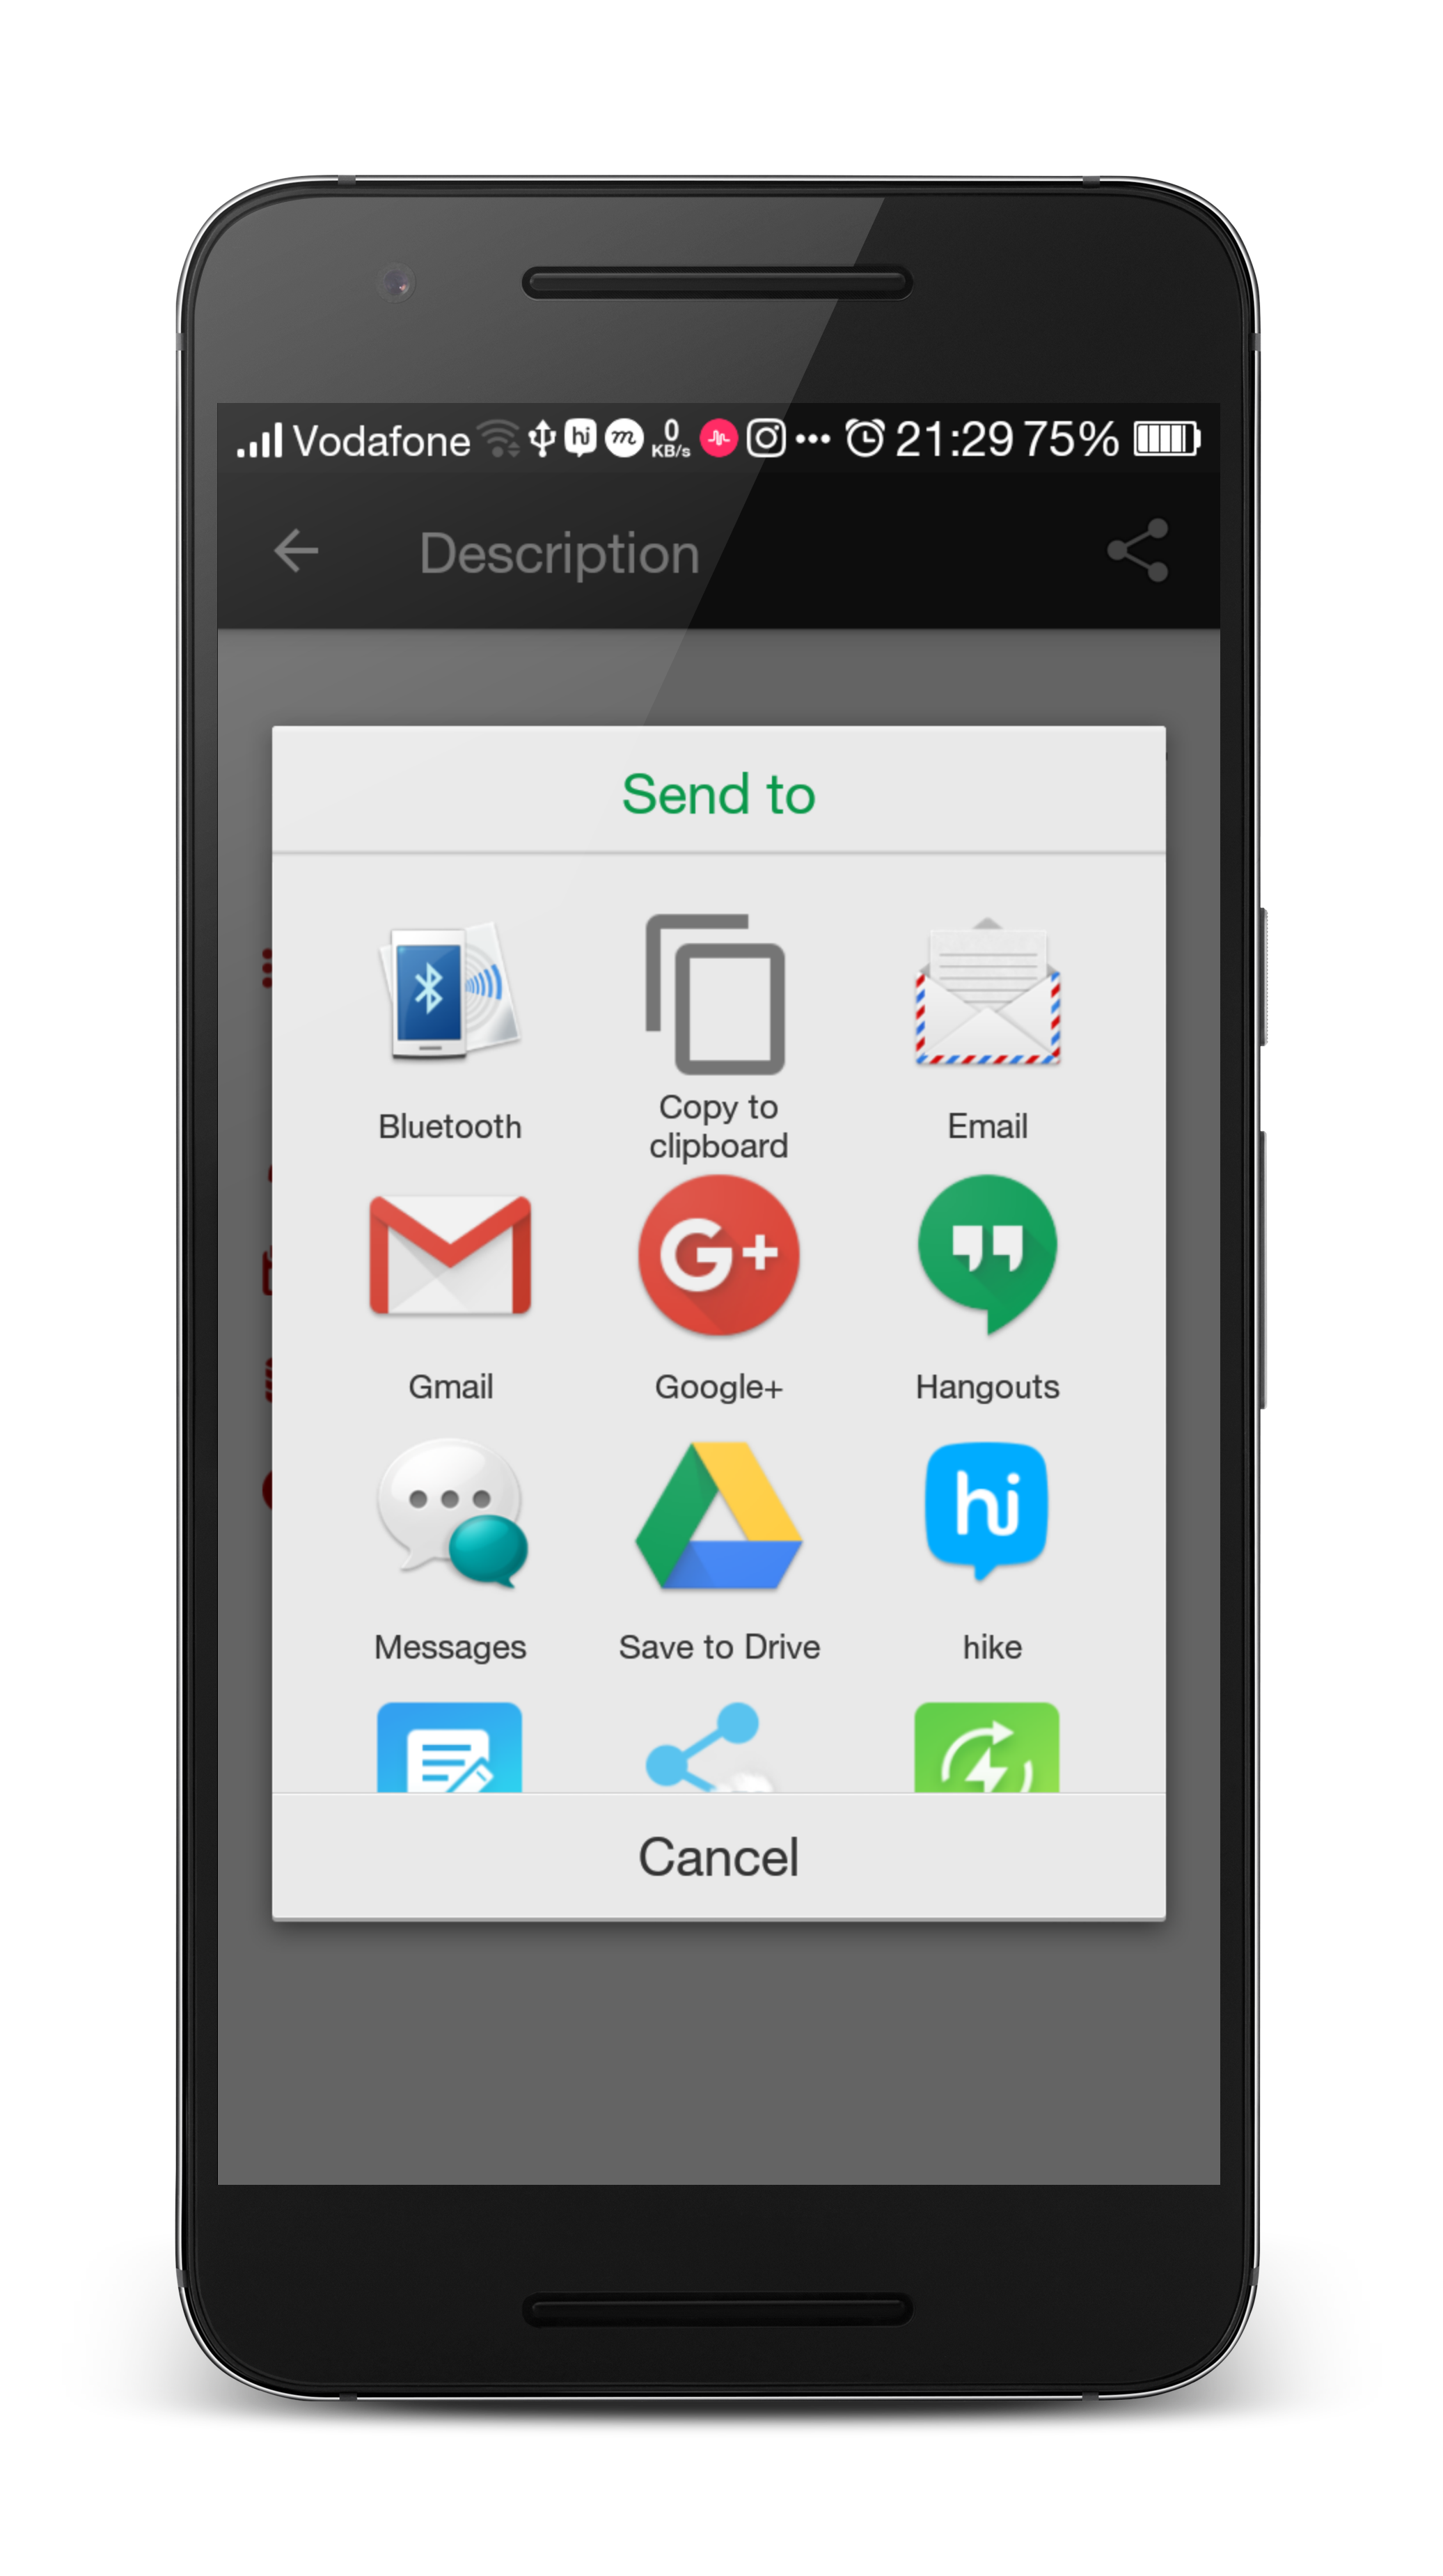
\includegraphics[scale=0.13]{images/d17.png}
\caption{Sharing Ebook}
\end{figure}

\newpage

\begin{figure}[ht]
\centering
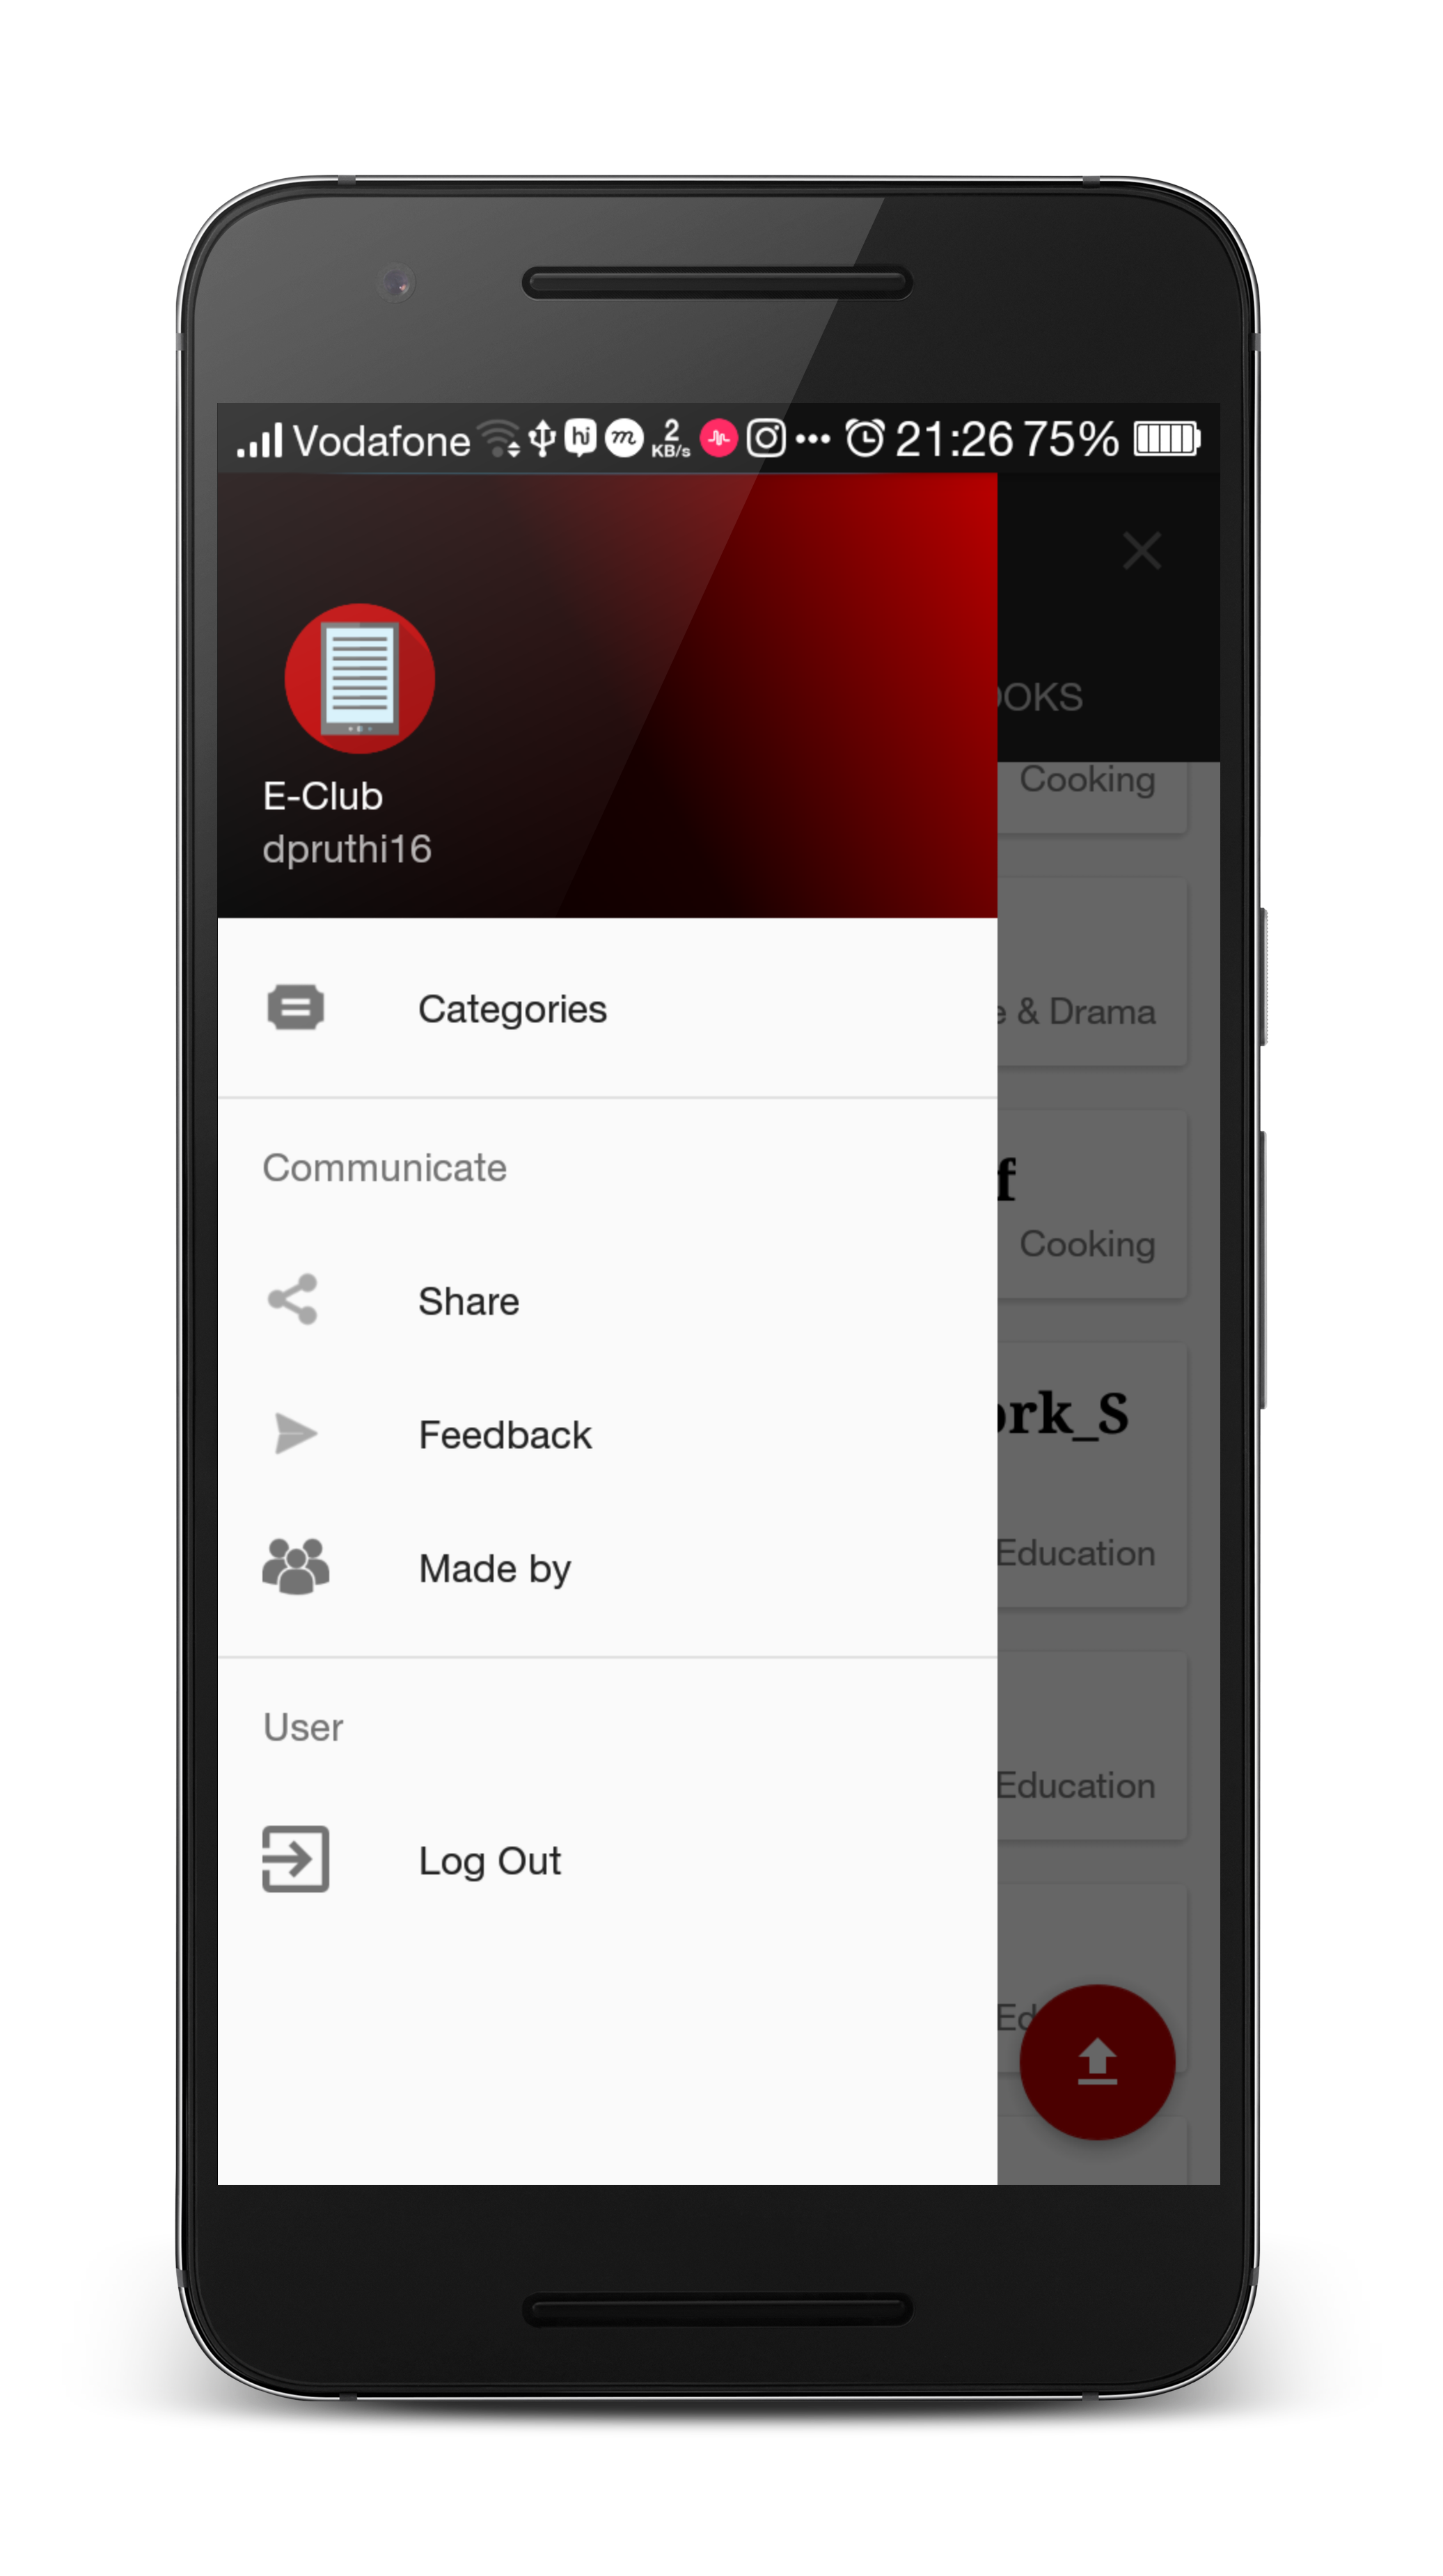
\includegraphics[scale=0.13]{images/d9.png}
\caption{Navigation Drawer}
\end{figure}

\newpage

\begin{figure}[ht]
\centering
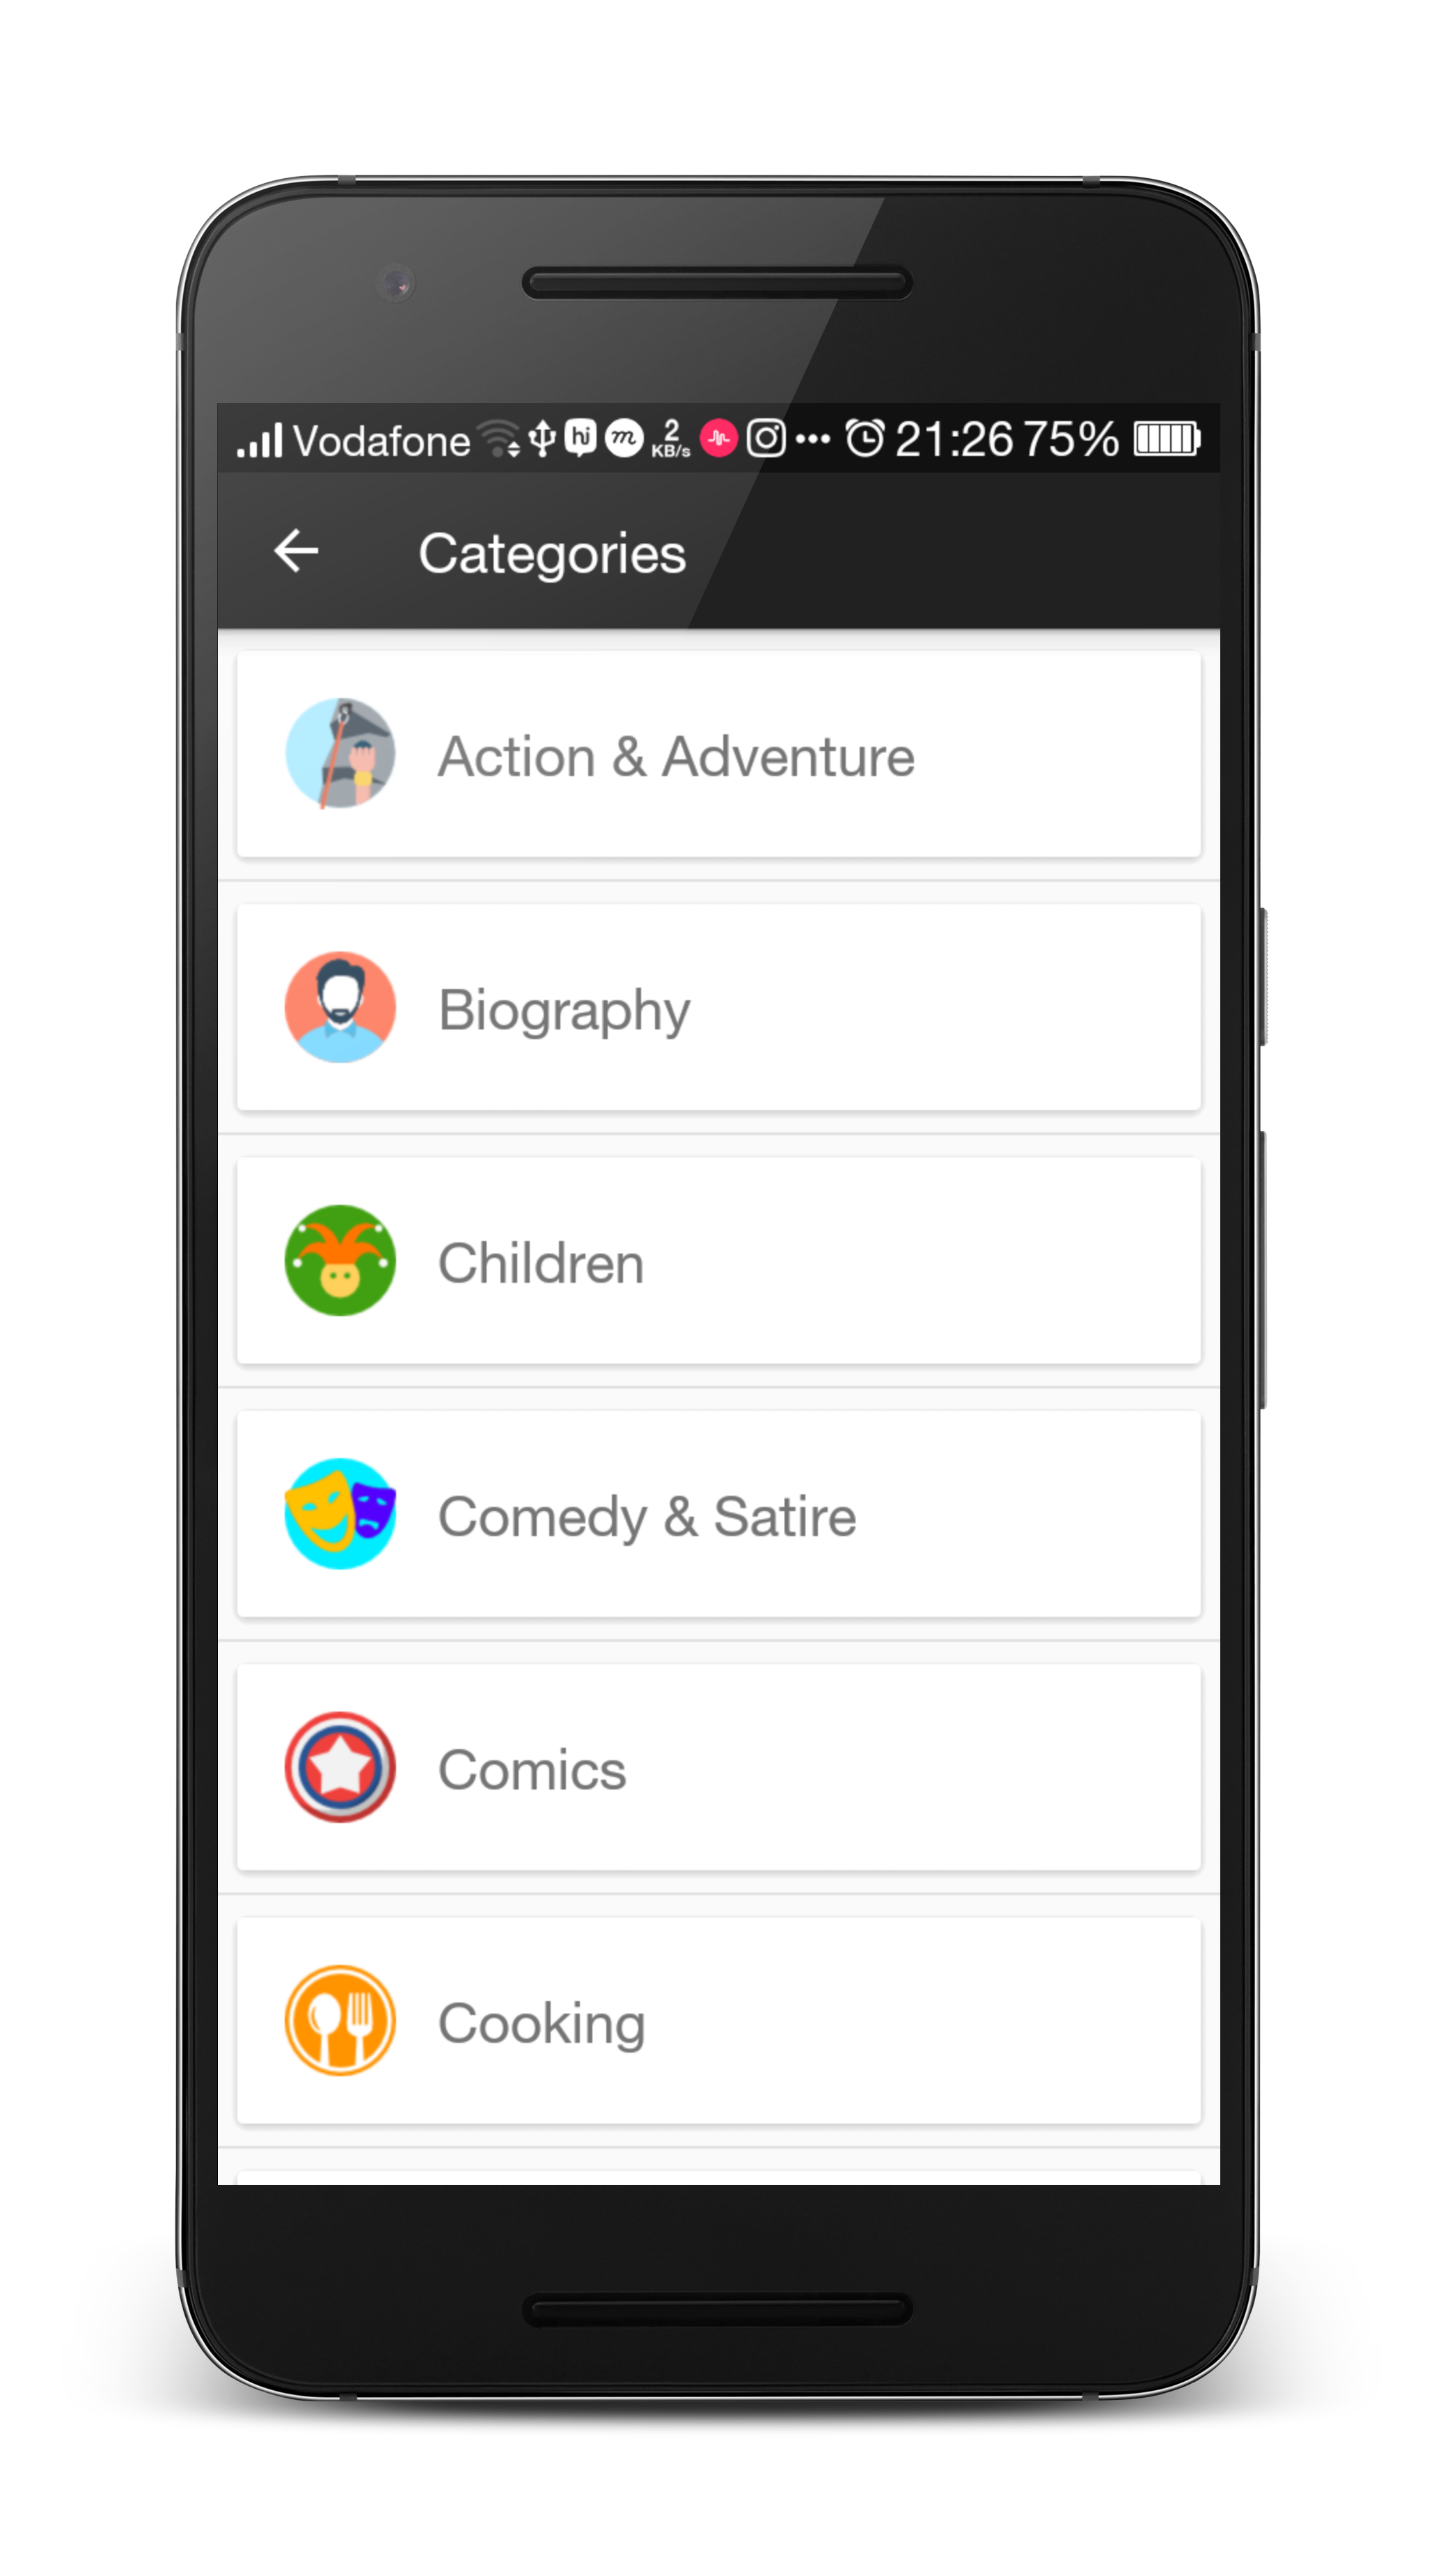
\includegraphics[scale=0.13]{images/d8.png}
\caption{Ebook Categories}
\end{figure}

\newpage

%\begin{figure}[ht]
%\centering
%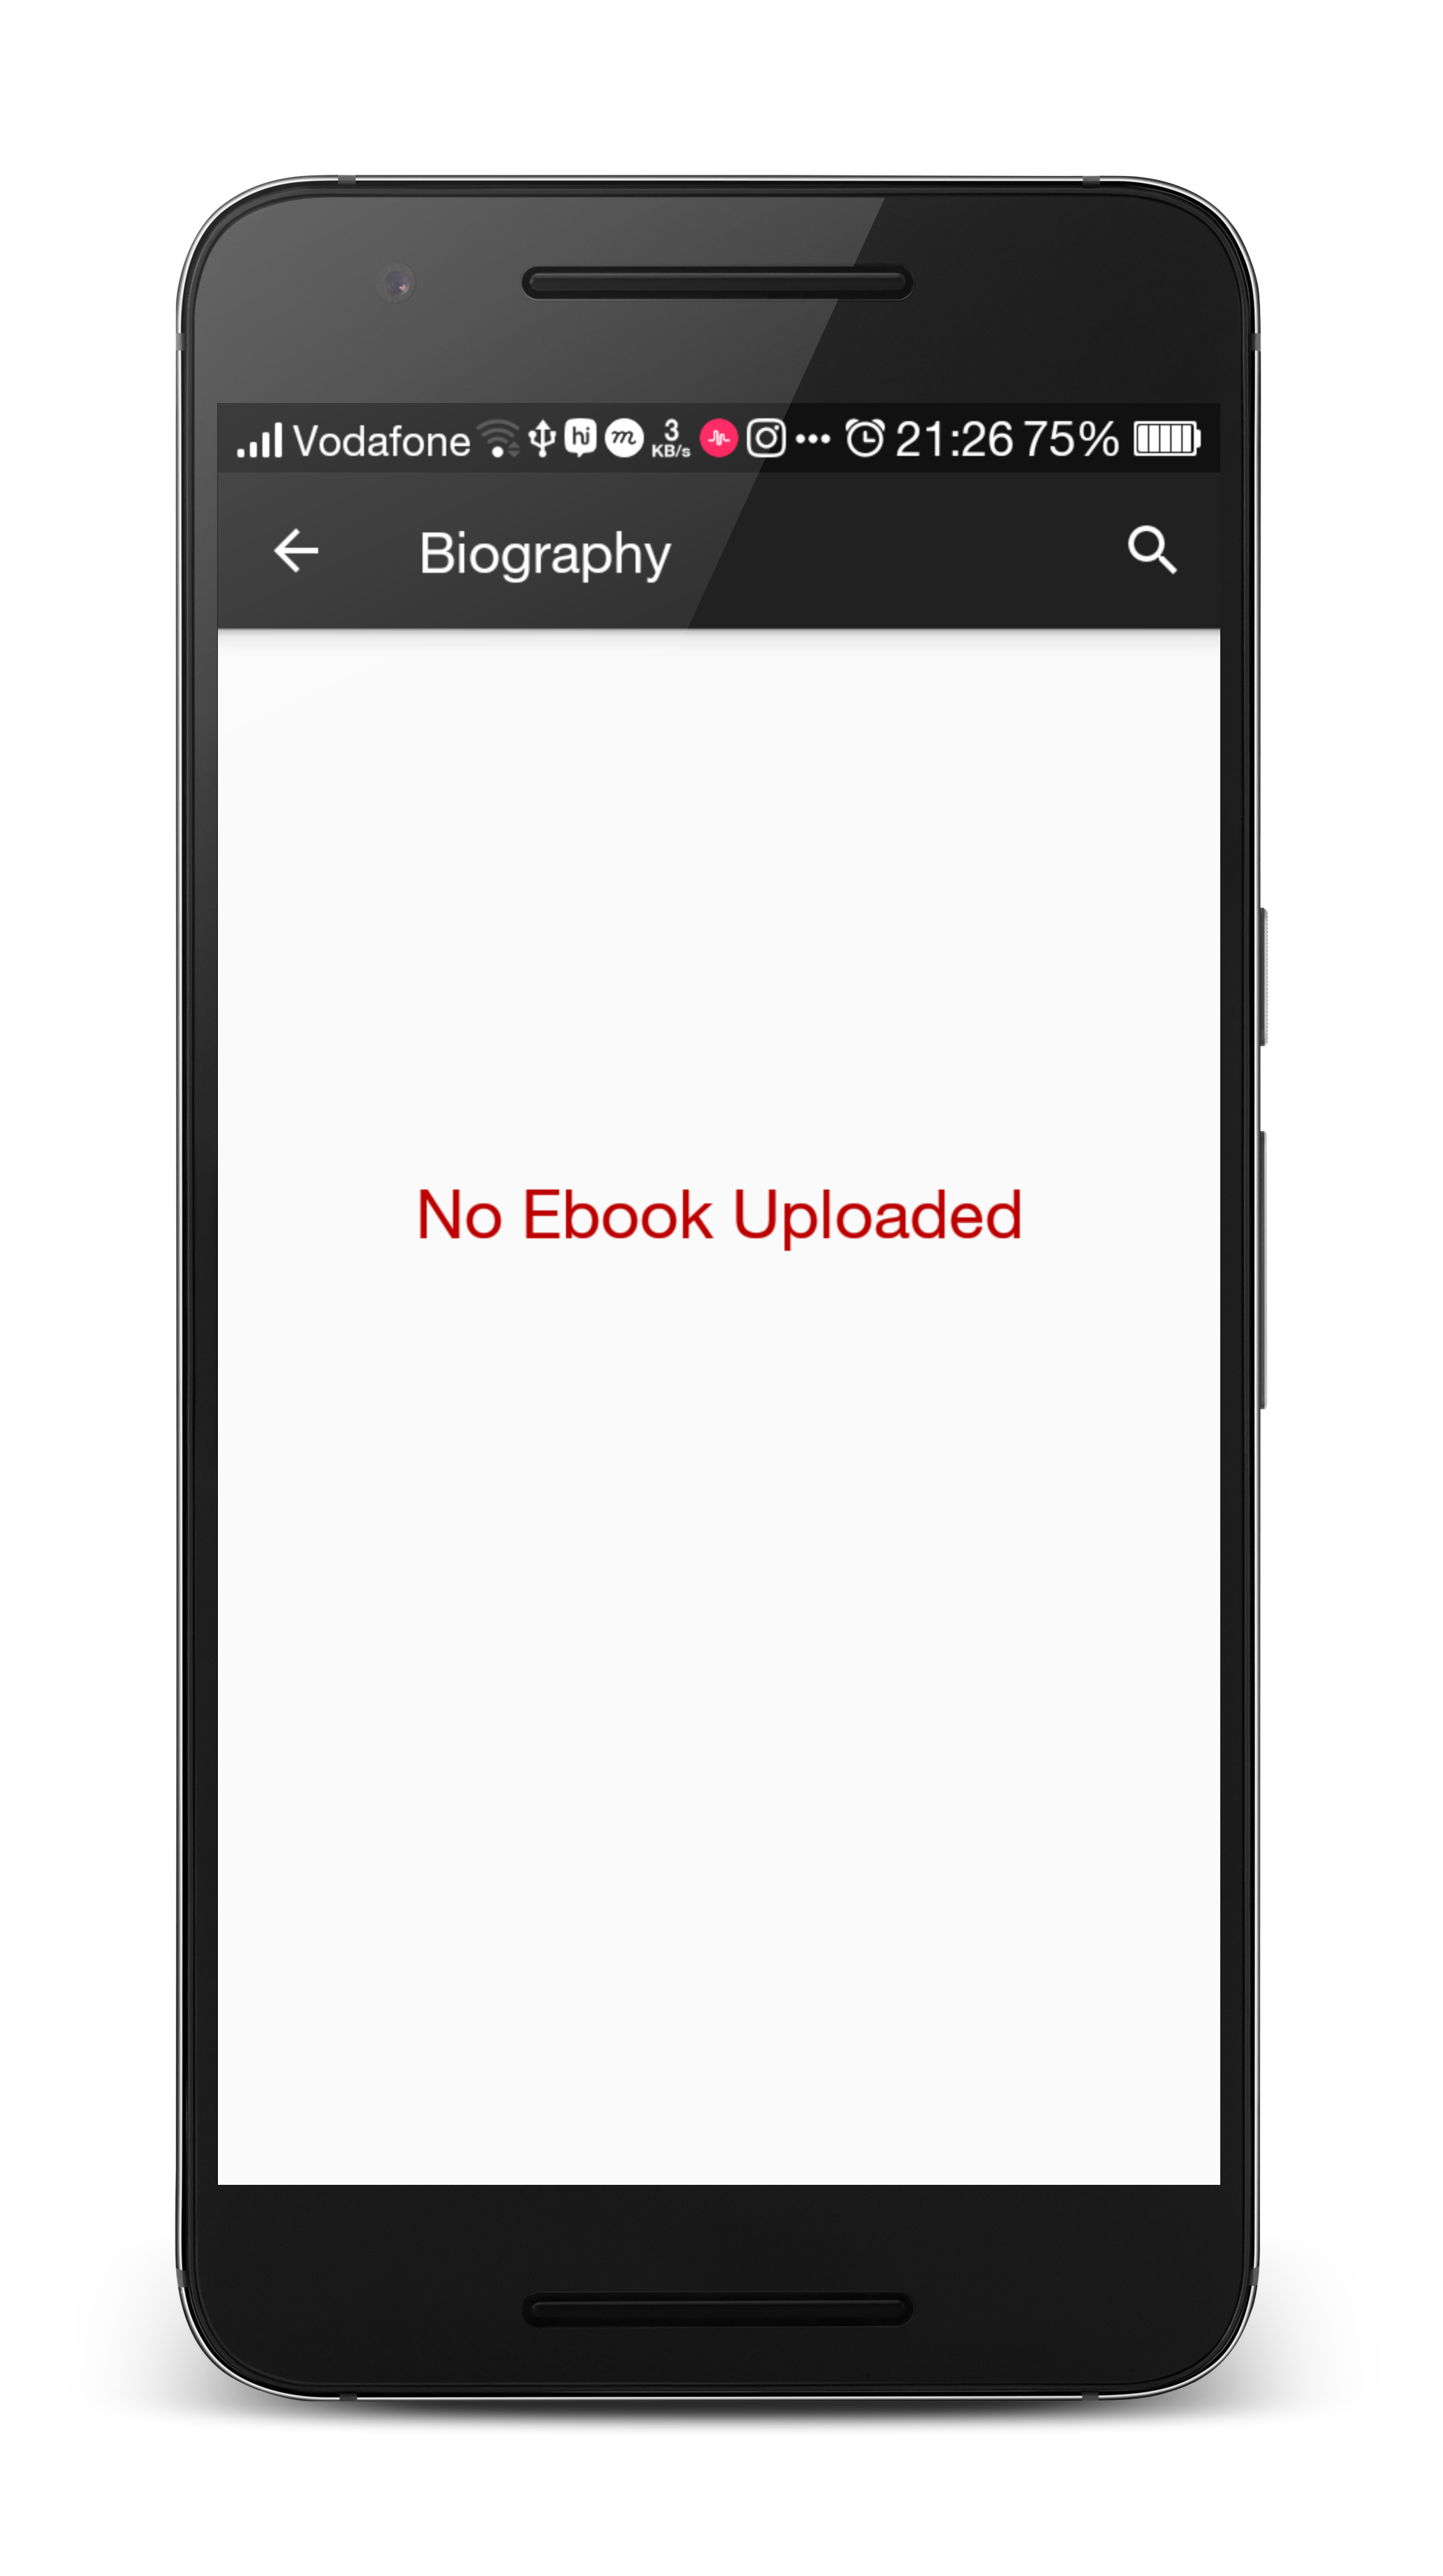
\includegraphics[scale=0.13]{images/d7.png}
%\caption{Screen 13}
%\end{figure}

%\newpage

%\begin{figure}[ht]
%\centering
%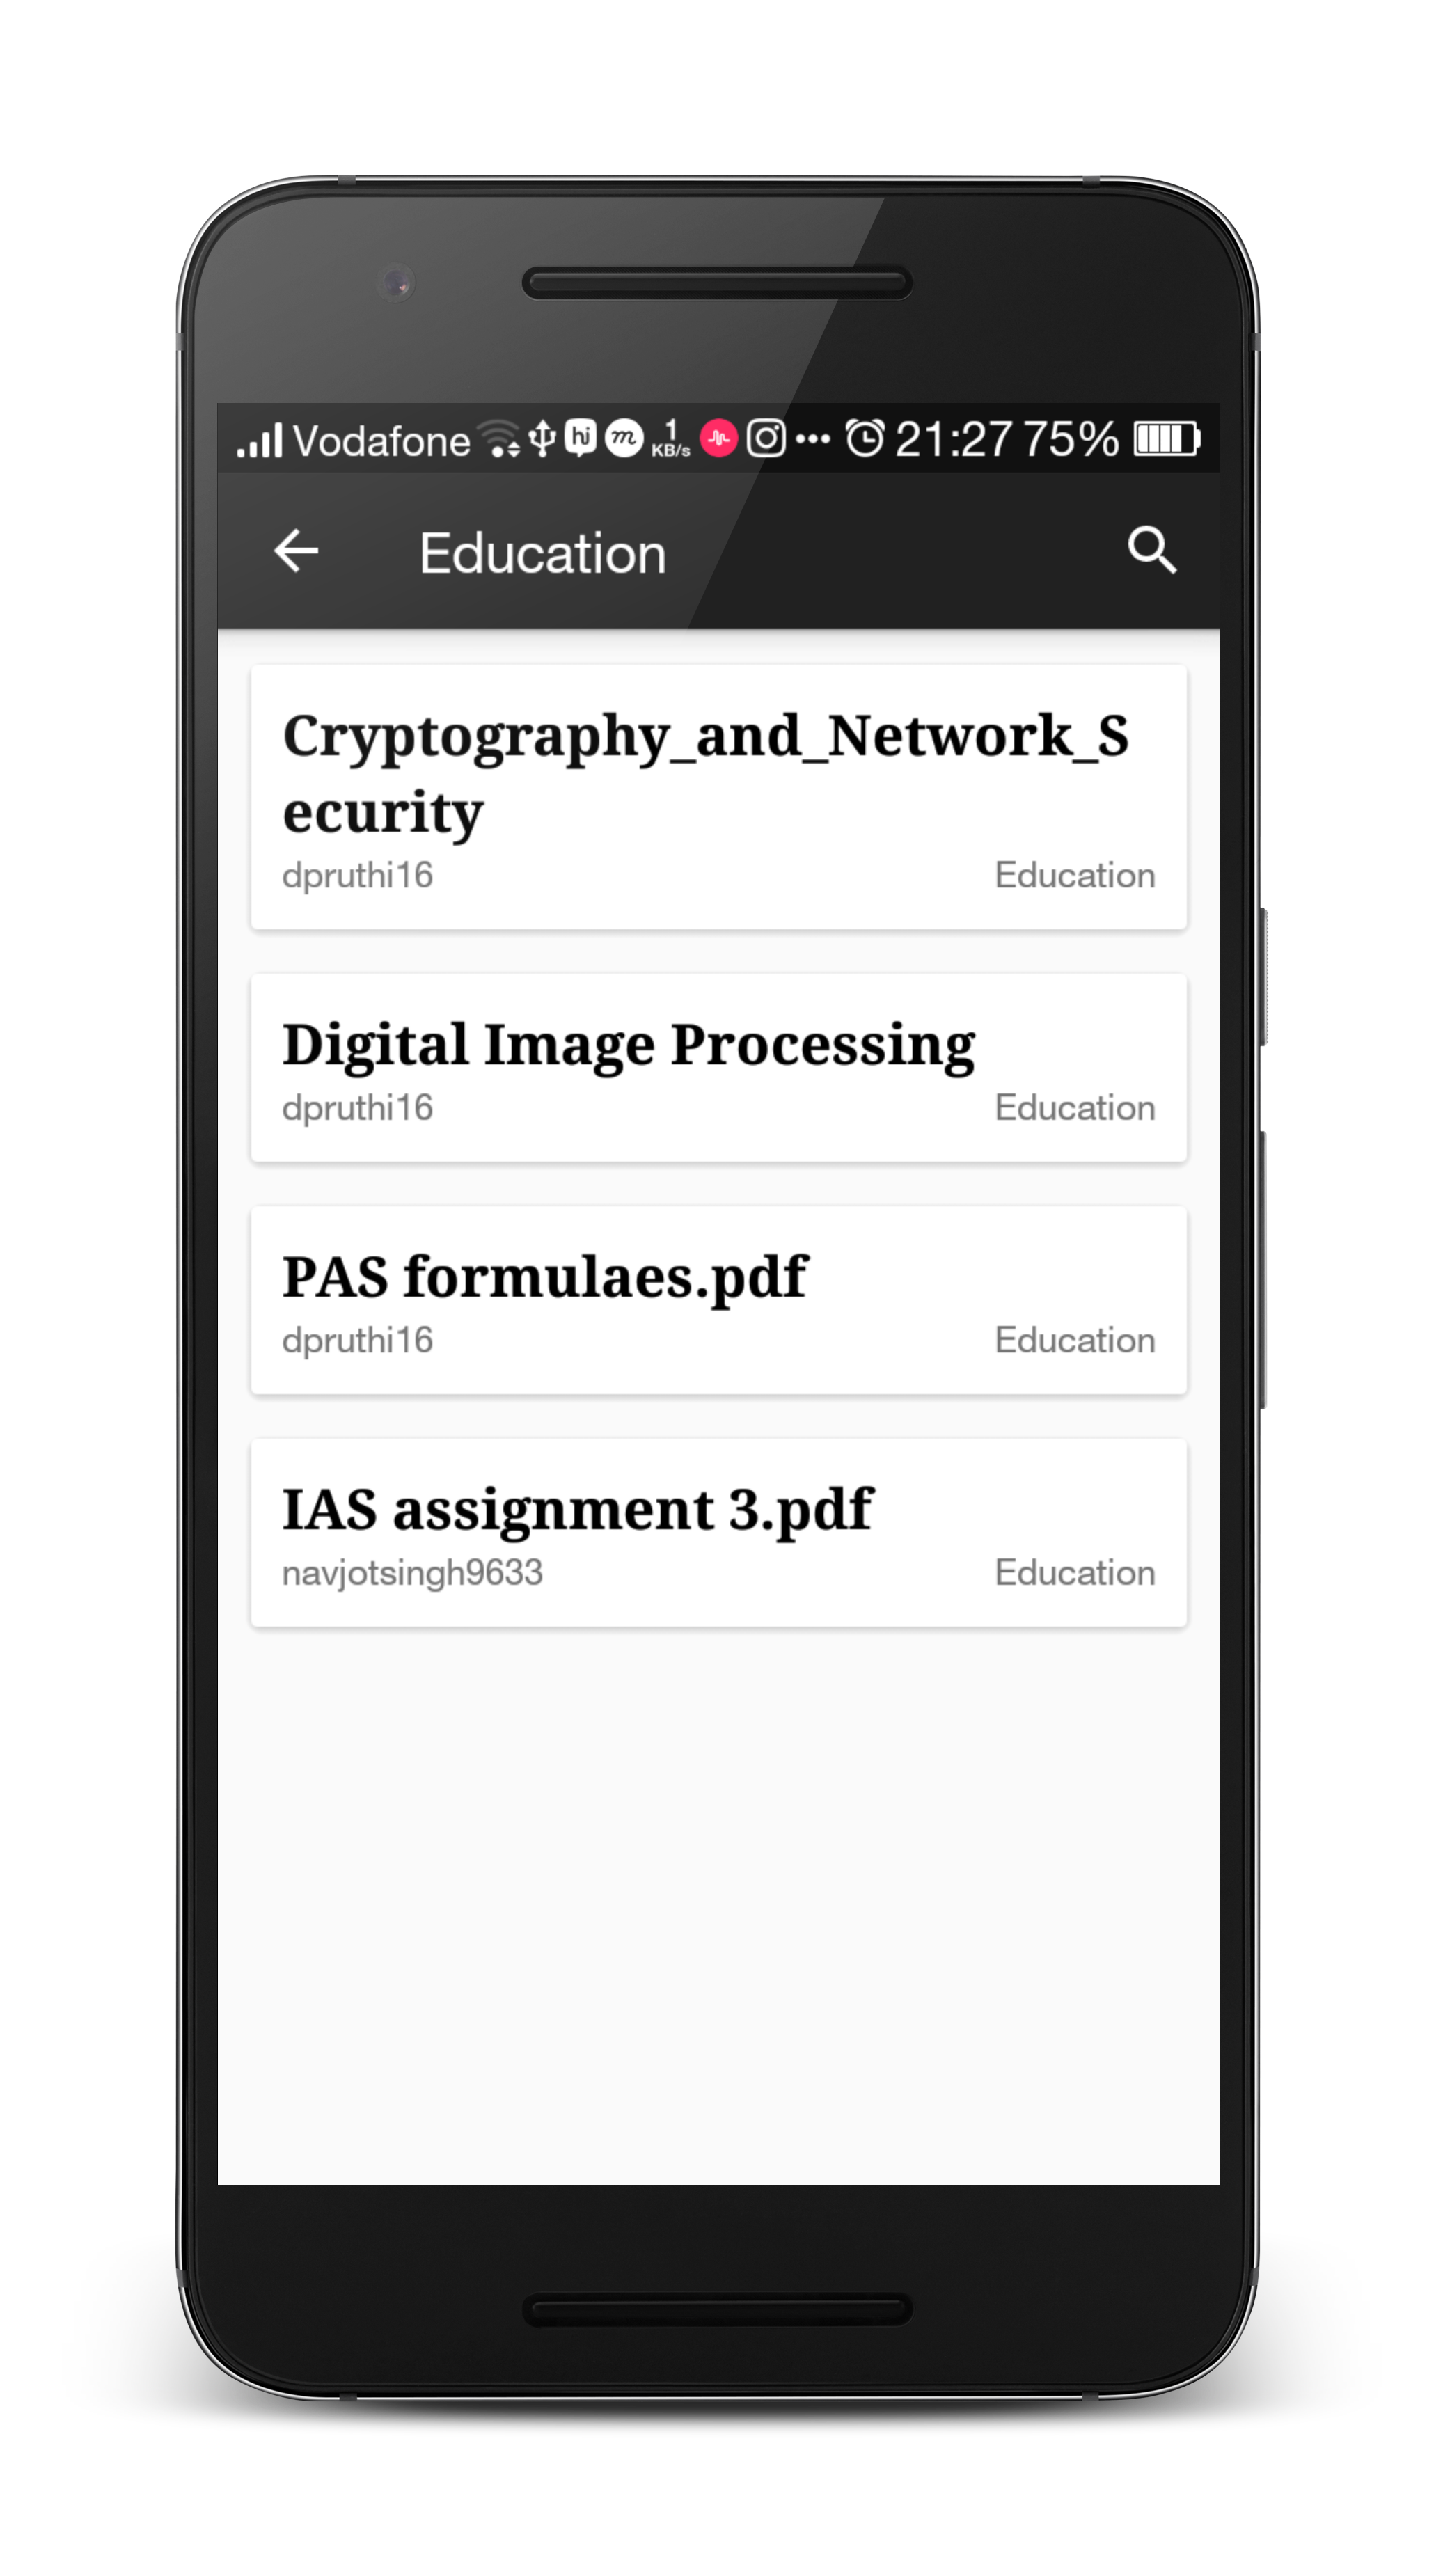
\includegraphics[scale=0.13]{images/d6.png}
%\caption{Screen 14}
%\end{figure}
%
%\newpage
\begin{figure}[ht]
\centering
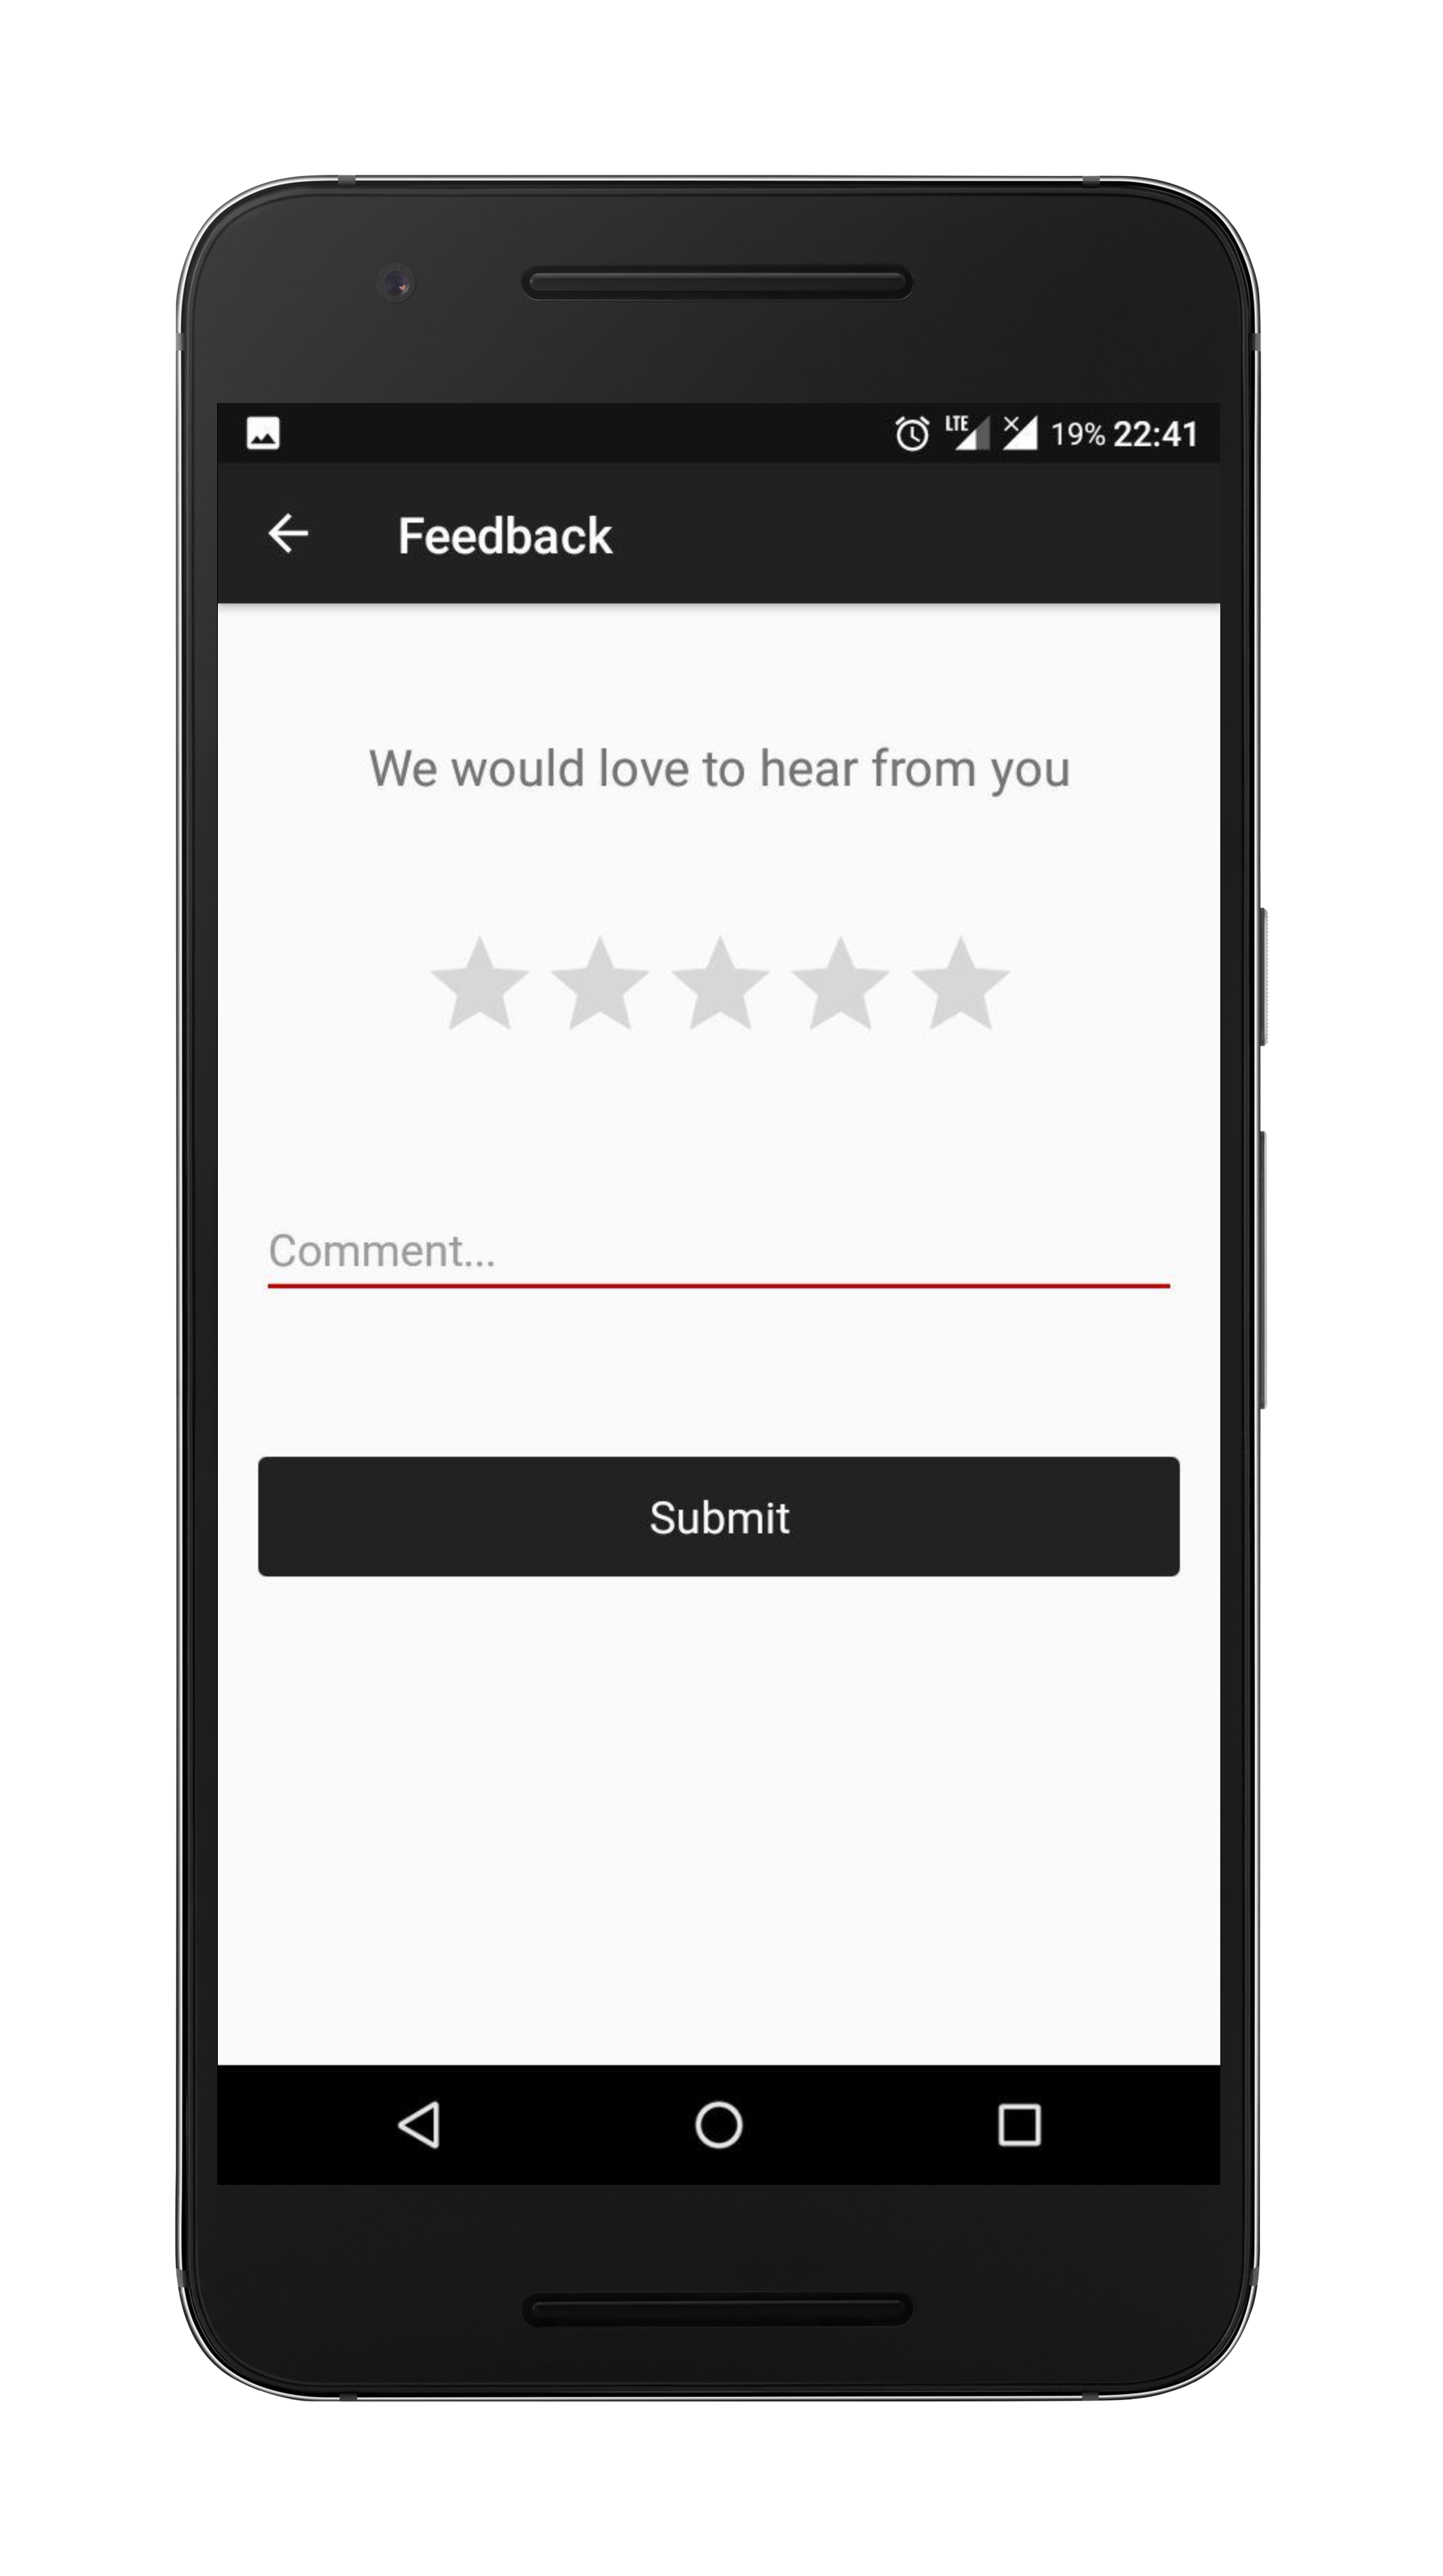
\includegraphics[scale=0.13]{images/f.png}
\caption{Feedback}
\end{figure}

\newpage
\begin{figure}[ht]
\centering
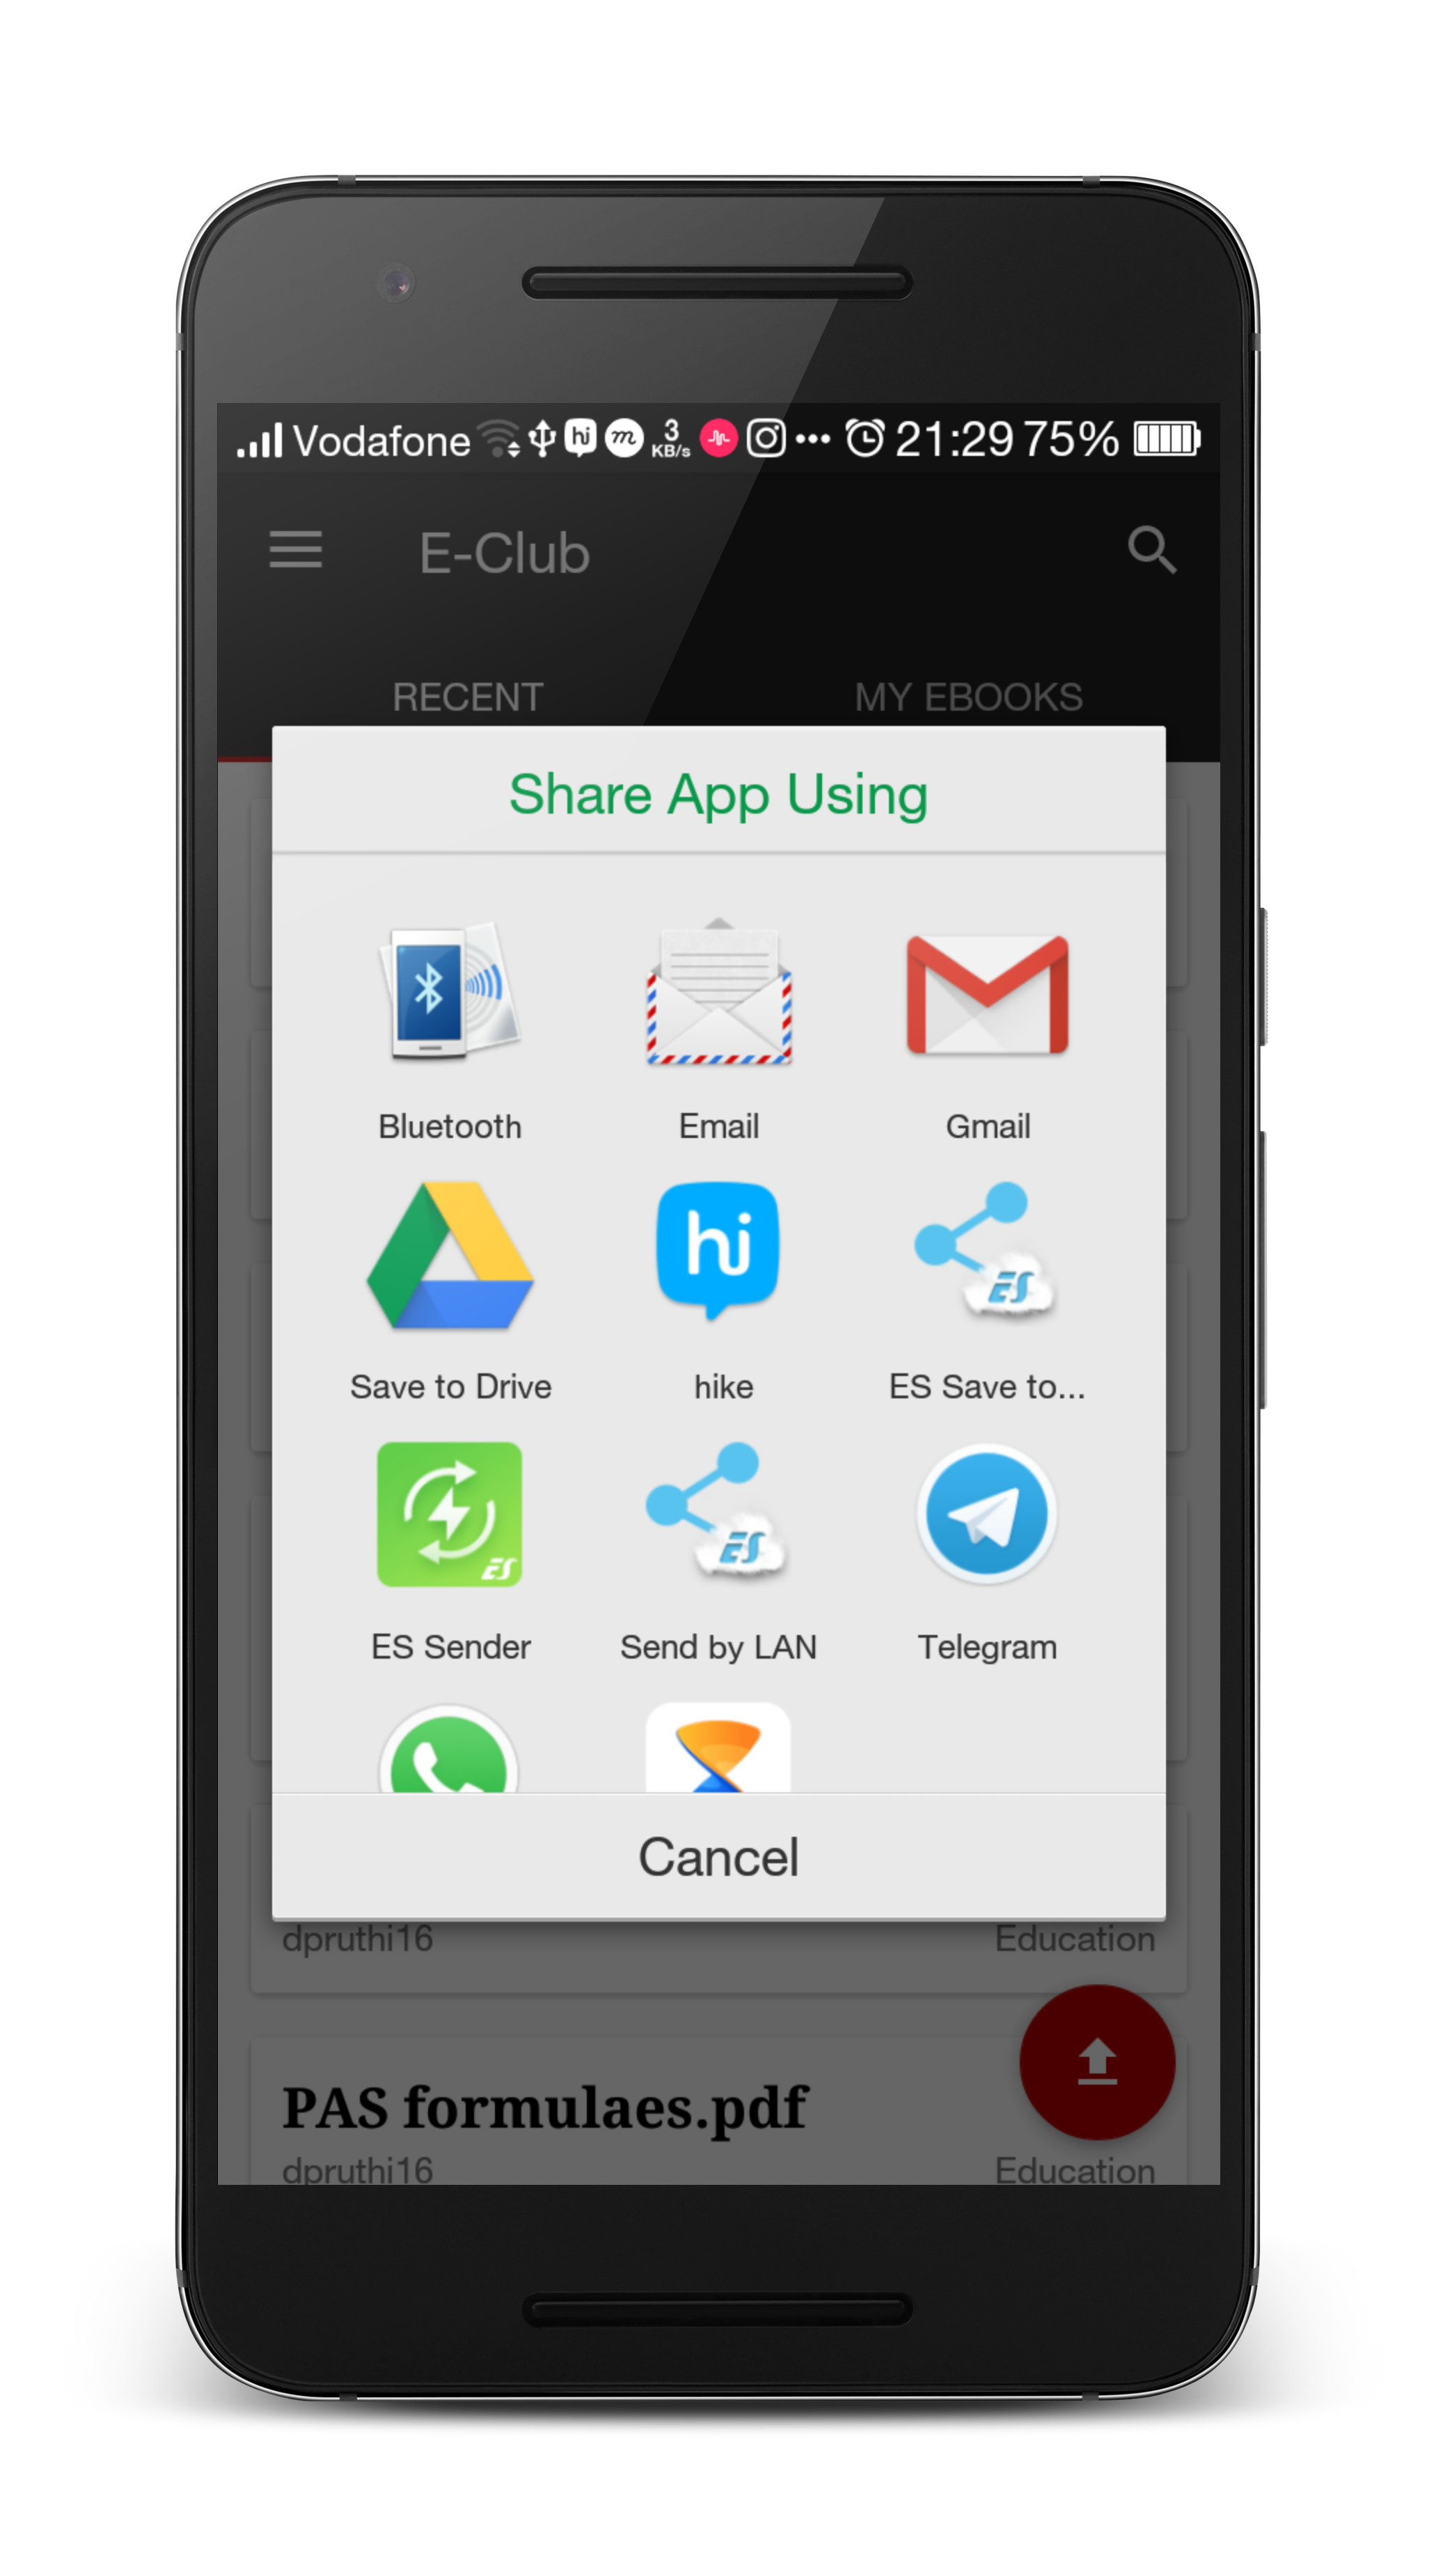
\includegraphics[scale=0.13]{images/d4.png}
\caption{Sharing App}
\end{figure}

\newpage
\begin{figure}[ht]
\centering
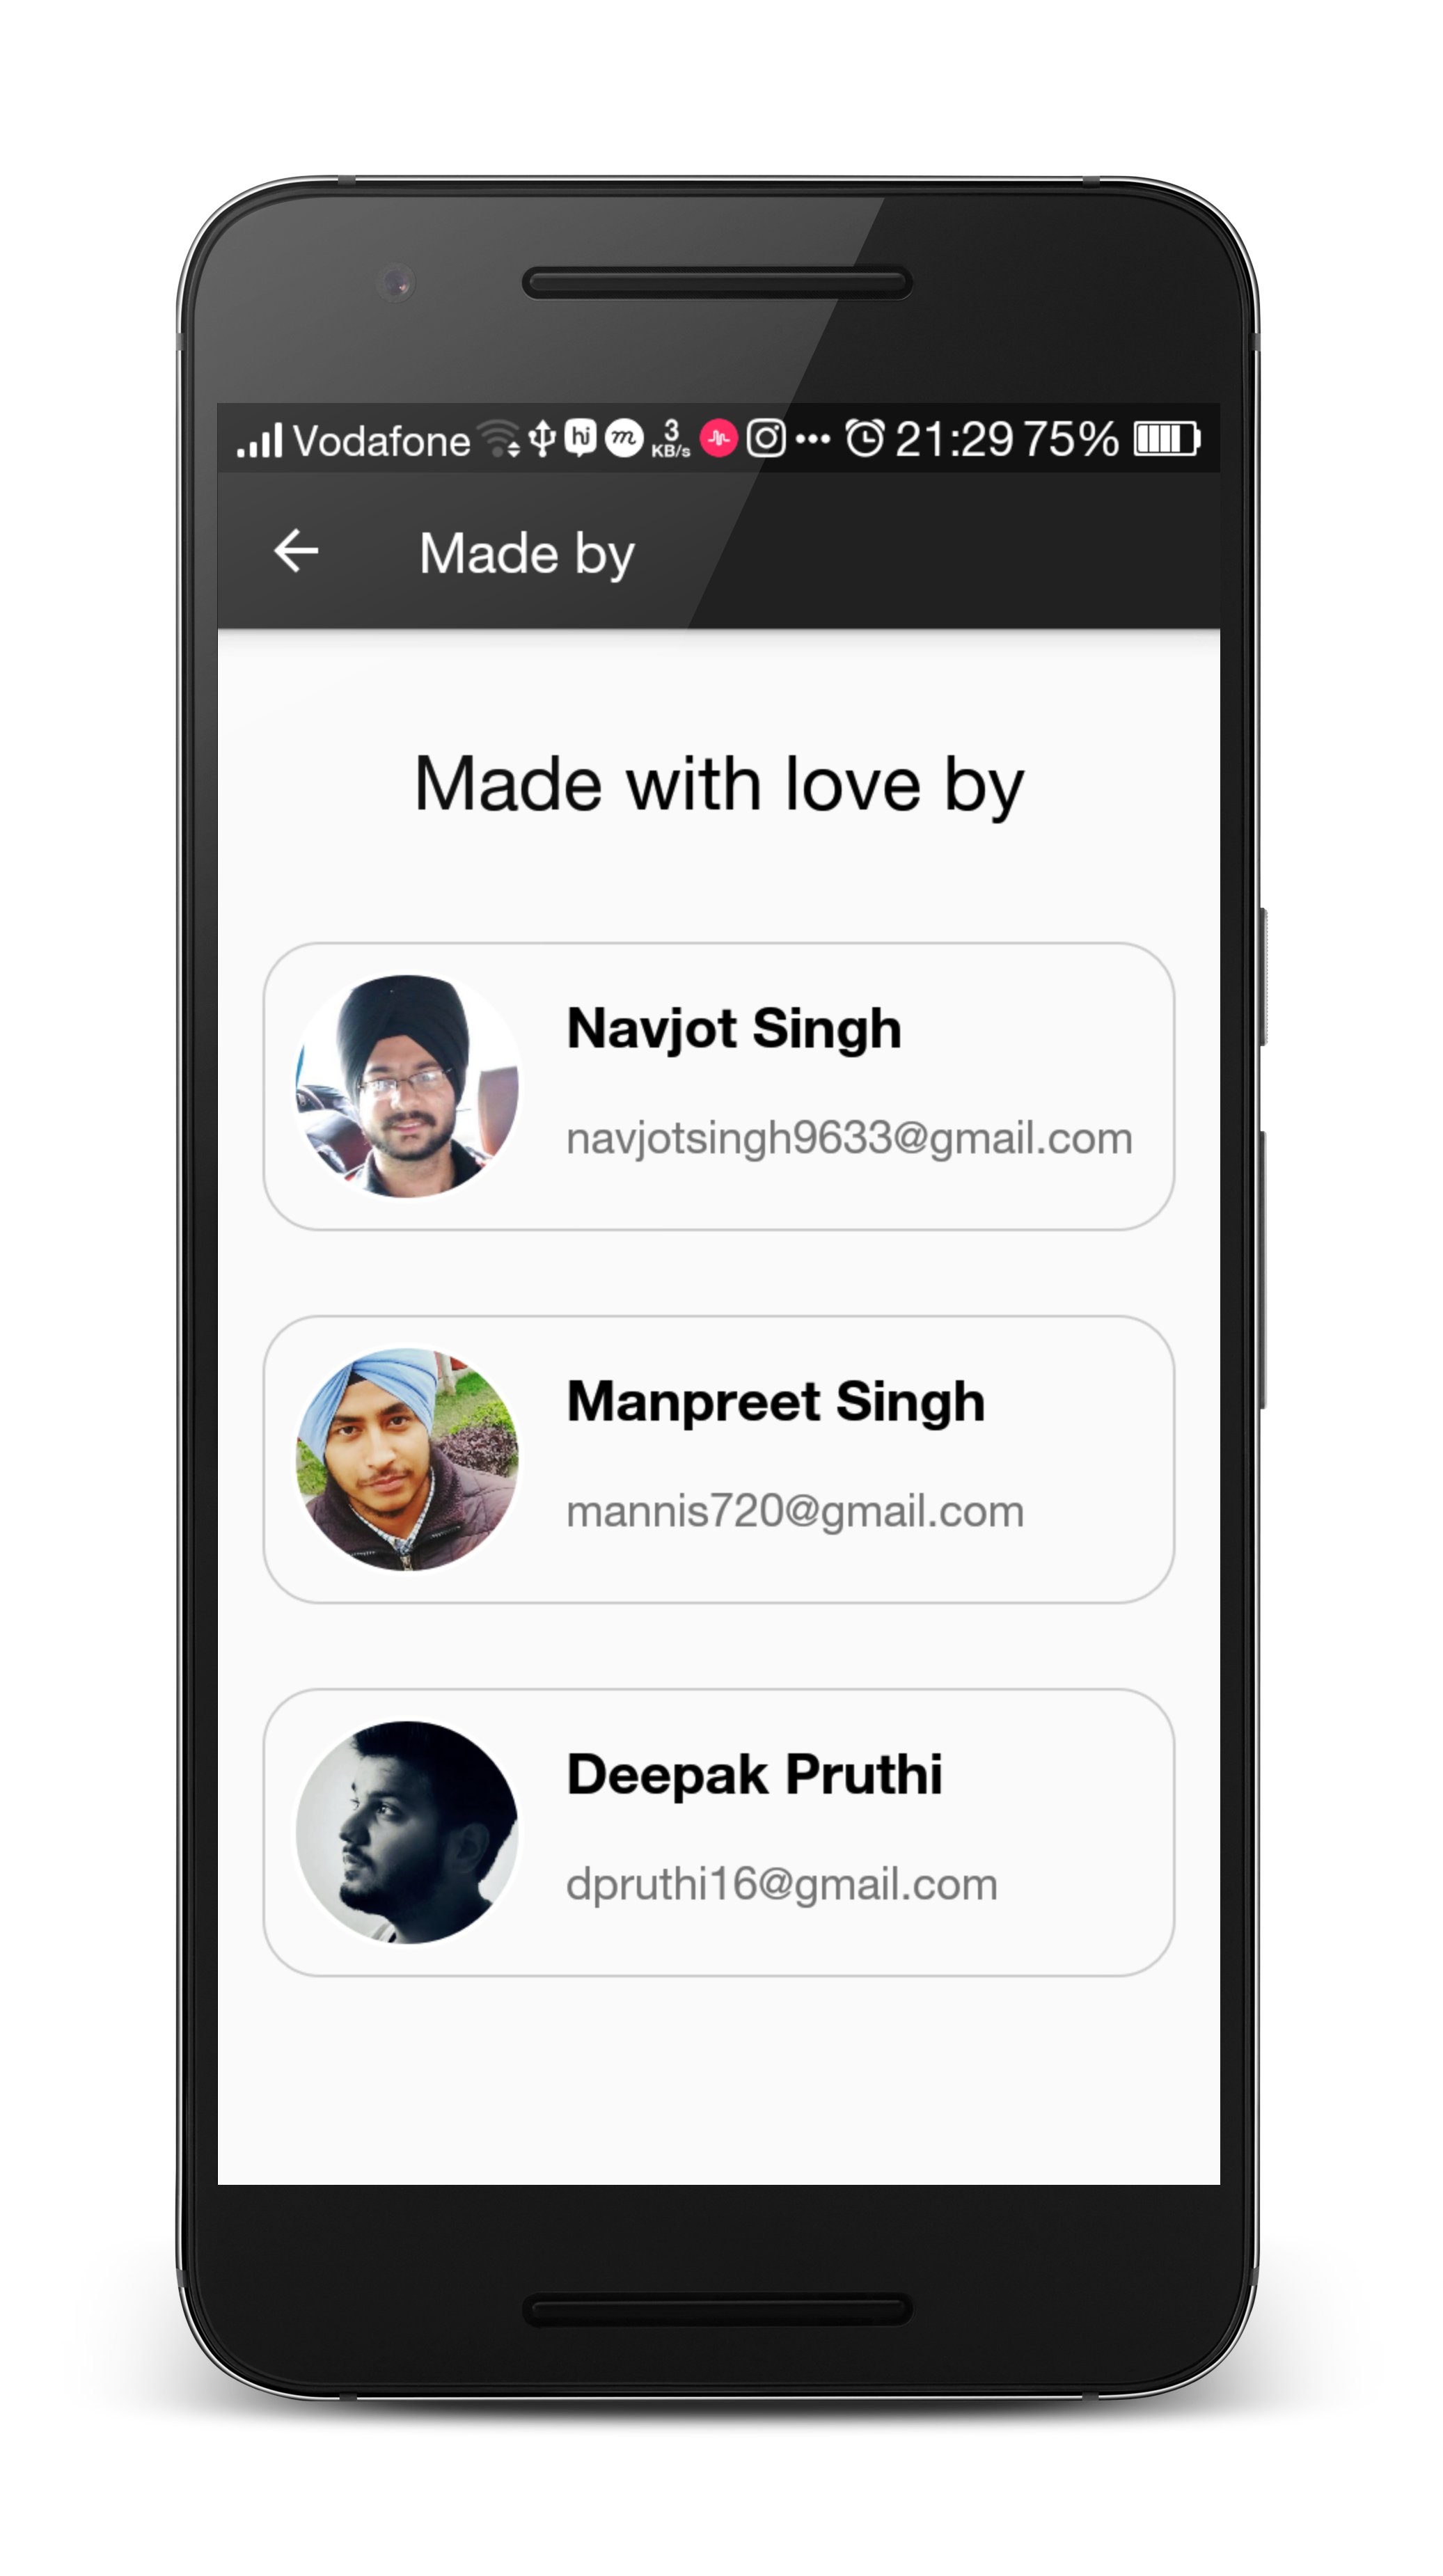
\includegraphics[scale=0.13]{images/d2.png}
\caption{Developers}
\end{figure}

\newpage

\section{Back Ends Representation}
\subsection{Firebase Realtime Database}
Store and sync data with our NoSQL cloud database. Data is synced across all clients in realtime, and remains available when your app goes offline.\\

The Firebase Realtime Database is a cloud-hosted database. Data is stored as JSON and synchronized in realtime to every connected client. When you build cross-platform apps with our iOS, Android, and JavaScript SDKs, all of your clients share one Realtime Database instance and automatically receive updates with the newest data.
\subsection{How does it work?}
The Firebase Realtime Database lets you build rich, collaborative applications by allowing secure access to the database directly from client-side code. Data is persisted locally, and even while offline, realtime events continue to fire, giving the end user a responsive experience. When the device regains connection, the Realtime Database synchronizes the local data changes with the remote updates that occurred while the client was offline, merging any conflicts automatically.\\

The Realtime Database provides a flexible, expression-based rules language, called Firebase Realtime Database Security Rules, to define how your data should be structured and when data can be read from or written to. When integrated with Firebase Authentication, developers can define who has access to what data, and how they can access it.\\

The Realtime Database is a NoSQL database and as such has different optimizations and functionality compared to a relational database. The Realtime Database API is designed to only allow operations that can be executed quickly. This enables you to build a great realtime experience that can serve millions of users without compromising on responsiveness. Because of this, it is important to think about how users need to access your data and then structure it accordingly.

\subsection{Snapshots of Database}

\begin{figure}[ht]
\centering
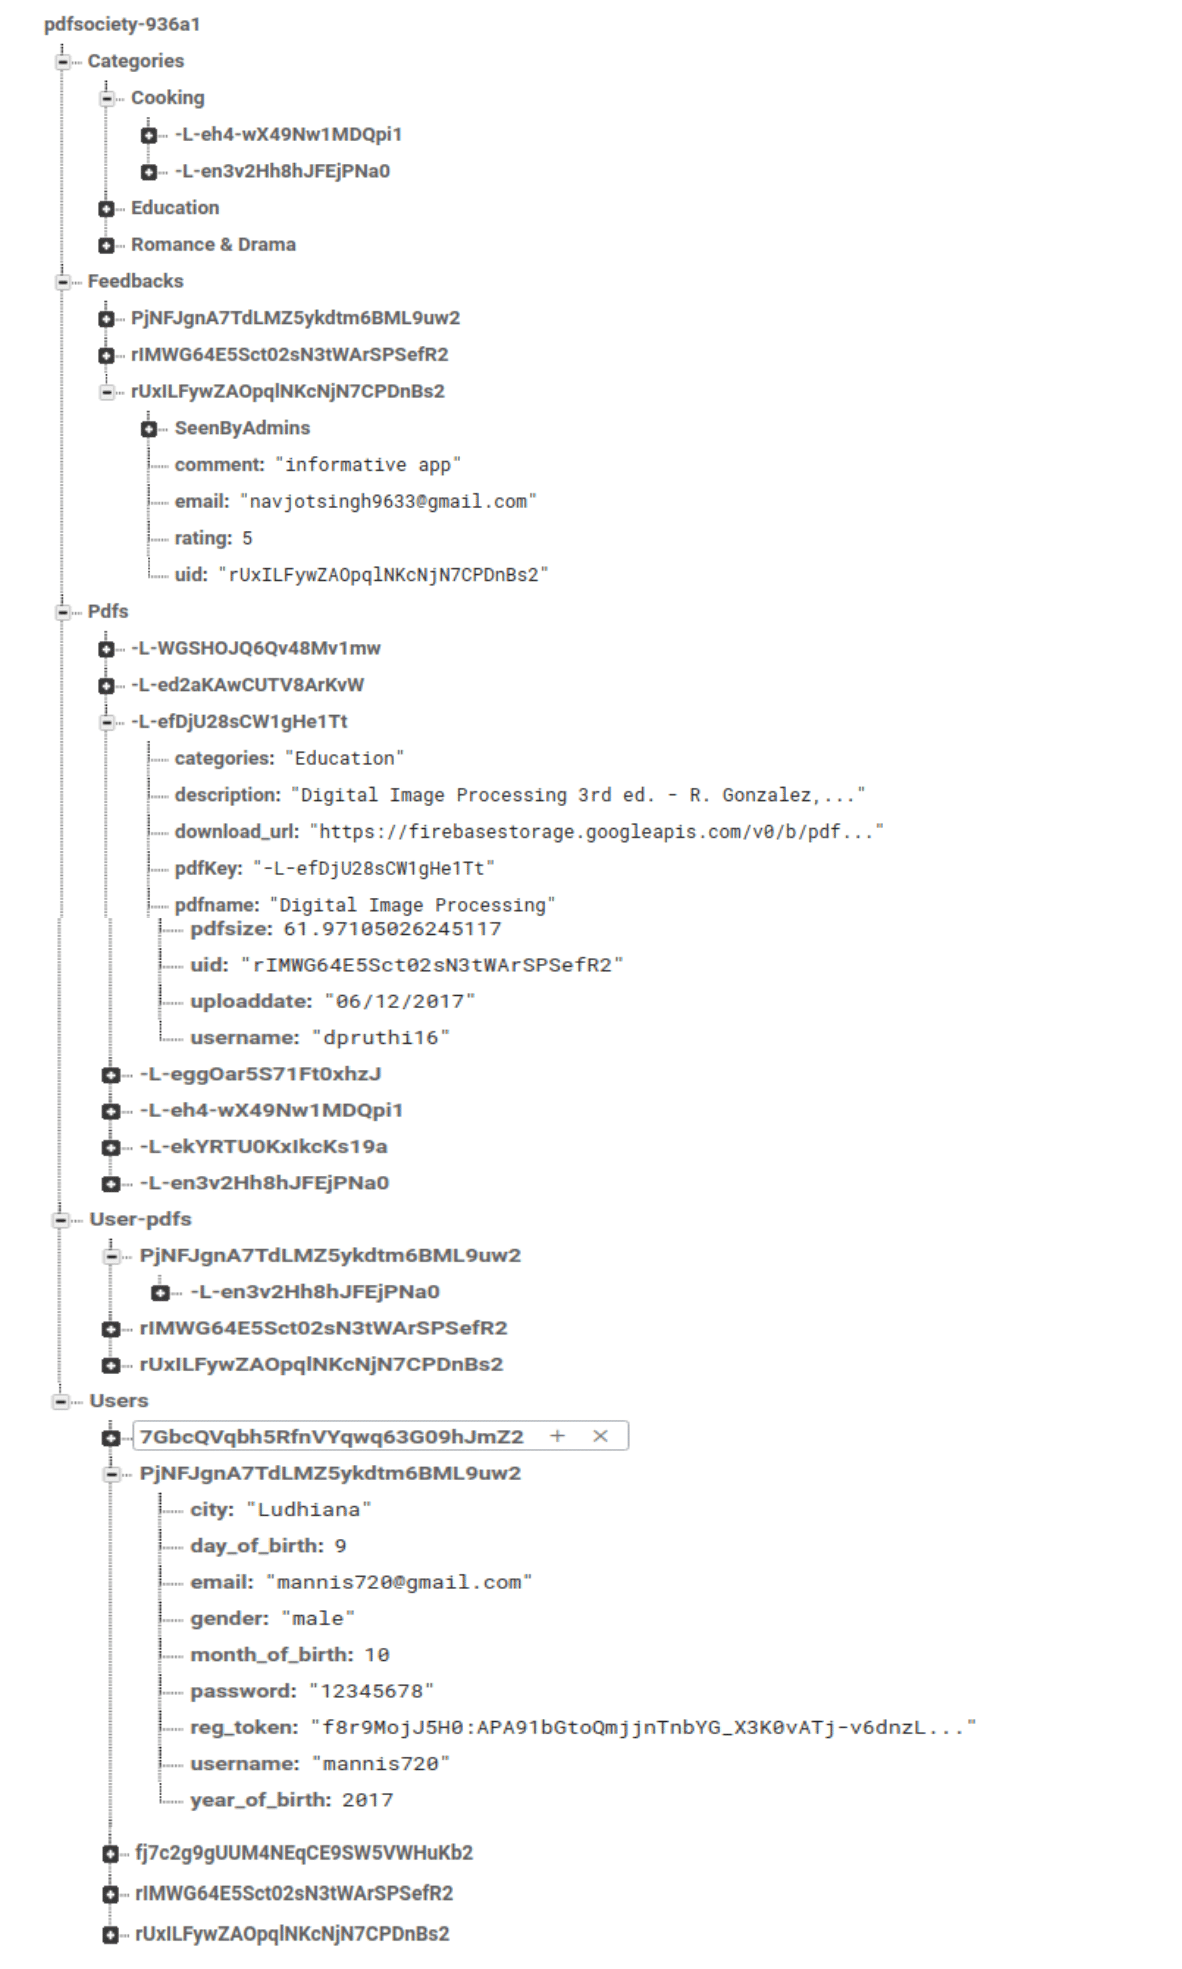
\includegraphics[scale=0.3]{images/dbb.png}
\caption{Database}
\end{figure}

